\documentclass[11pt,a4paper,titlepage]{article}

\usepackage[margin=0.8in, top=0.9in, bottom=0.9in]{geometry}
\usepackage{graphicx}
\usepackage{amsmath}
\usepackage{amssymb}
\usepackage{fancyhdr}
\usepackage{color}
\usepackage{url}
\usepackage{array}
\usepackage{tabularx}

% Define color palette
\definecolor{navy}{rgb}{0.0, 0.18, 0.39}
\definecolor{darkred}{rgb}{0.65, 0.1, 0.1}
\definecolor{darkgreen}{rgb}{0.1, 0.45, 0.1}
\definecolor{darkgray}{rgb}{0.25, 0.25, 0.25}
\definecolor{lightgray}{rgb}{0.92, 0.92, 0.92}

% Header and Footer configuration
\pagestyle{fancy}
\fancyhf{}
\lhead{\small \textcolor{darkgray}{MiniBass: Algorithmic Design and Comparative Analysis}}
\rhead{\small \textcolor{darkgray}{$10 \times 12\text{ m}$ Performance Venue}}
\cfoot{\small \thepage}
\renewcommand{\headrulewidth}{0.4pt}
\renewcommand{\footrulewidth}{0.2pt}

\newenvironment{proof}{\noindent\textbf{Proof.}}{\hfill$\blacksquare$\vspace{0.5em}\par}

\begin{document}

% ==============================================================================
% FORMAL COVER PAGE
% ==============================================================================
\begin{titlepage}
    \centering
    \vspace*{1.5cm}
    
    {\Large \textbf{Title:}}\\[0.6em]
    {\Huge \bfseries \textcolor{navy}{MiniBass: Low-Frequency Sound Field Optimization and Multi-Source Active Control}}\\[2.0cm]
    
    {\Large \textbf{Project:}}\\[0.6em]
    {\LARGE Multi-Subwoofer Acoustic Field Synthesis and Algorithmic Optimization in Enclosed Performance Venues}\\[2.0cm]
    
    {\Large \textbf{Course Code:}}\\[0.6em]
    {\LARGE [Course Code]}\\[2.0cm]
    
    \vfill
    
    \begin{minipage}{0.85\textwidth}
        \centering
        {\Large \textbf{Presented to:}}\\[0.6em]
        {\LARGE [Instructor Name / Department]}\\[2.5cm]
        
        \begin{tabular}{rl}
            \Large \textbf{Name:} & \Large [Student Name] \\[1.0em]
            \Large \textbf{Reg Number:} & \Large [Registration Number] \\
        \end{tabular}
    \end{minipage}
    
    \vspace*{1.5cm}
\end{titlepage}

% ==============================================================================
% TABLE OF CONTENTS & LISTS
% ==============================================================================
\pagenumbering{roman}
\tableofcontents
\newpage
\listoffigures
\vspace{1.0em}
\listoftables
\newpage

% ==============================================================================
% EXECUTIVE SUMMARY
% ==============================================================================
\section*{Executive Summary}
\addcontentsline{toc}{section}{Executive Summary}

Low-frequency sound reproduction ($20\text{--}200\text{ Hz}$) inside enclosed rectangular halls is fundamentally degraded by standing wave boundary reflections. These room modes generate severe spatial variations in sound pressure level (SPL), leaving individual audience seats subject to constructive peaks ($+10\text{ to }+15\text{ dB}$) or deep non-minimum-phase interference notches ($-15\text{ to }-25\text{ dB}$). Because these notches arise from destructive spatial interference rather than transducer deficiencies, global electrical equalization cannot resolve them without driving other seats into excessive resonance.

This report presents a thorough investigation into the design, computational structure, empirical performance, and physical field behavior of \textbf{four distinct optimization algorithms} developed to synthesize multi-source bass arrays along the front stage of a $10.0 \times 12.0 \times 2.8\text{ m}$ performance venue ($V = 336\text{ m}^3$, $T_{60} = 0.45\text{ s}$). Rather than treating acoustic optimization as a single-objective black box, four differing algorithmic paradigms are formulated, executed, and benchmarked on identical physical data:
\begin{enumerate}
    \item \textbf{Algorithm 0: Layered Beam Search Optimizer} (Heuristic multi-objective discrete search with beam width $W=32$ and Pareto filtering across RMS error, power, and enclosure displacement).
    \item \textbf{Algorithm 1: Vectorized Geometric Tensor Scanner} (High-throughput SIMD tensor evaluator directly maximizing the pooled audience cell pass rate within a $\pm 3.0\text{ dB}$ tolerance corridor).
    \item \textbf{Algorithm 2: Multi-Seat Minimax Optimizer} (Audience fairness formulation maximizing the worst-seat passing frequency count $\max \min_s k_s$ and minimizing peak single-seat deviation).
    \item \textbf{Algorithm 3: RLT Active Bilinear Boundary Solver} (Reformulation-Linearization Technique decomposing quadratic acoustic interference into self and cross terms to synthesize active boundary absorption dipoles).
\end{enumerate}

To ensure complete scientific rigor and avoid over-fitting, all four algorithms are evaluated across both \textbf{80 in-sample listener seats} and an independent partition of \textbf{40 held-out off-grid verification seats} across 95 discrete frequencies ($20\text{--}200\text{ Hz}$), as well as a dense continuous room field grid ($25 \times 30 = 750\text{ points}$). 

The benchmark proves that \textbf{no single algorithm dominates across all acoustic dimensions}:
\begin{itemize}
    \item \textbf{Algorithm 0} achieves the lowest room-wide RMS flatness error ($6.25\text{ dB}$ in-sample, $6.16\text{ dB}$ held-out), delivering the flattest global energy response.
    \item \textbf{Algorithm 1} maximizes total audience cell compliance within the $\pm 3.0\text{ dB}$ corridor ($43.32\%$ in-sample, $41.47\%$ held-out), capturing 307 additional seat-tone cells over Algorithm 0.
    \item \textbf{Algorithm 2} establishes superior audience fairness: every seat in the audience passes at least 24 discrete frequencies (compared to 10 for Algorithm 0 and 0 for Algorithm 3), while simultaneously cutting held-out worst-seat error to $9.48\text{ dB}$.
    \item \textbf{Algorithm 3} operates as an active boundary absorber: by synthesizing an active phase-inverted dipole pair at stage center, it destructively absorbs $55.7\%\text{--}68.3\%$ of boundary modal cross-term energy while drawing only $1.95\text{ W}$ mean electrical power per tone (a $52\%$ reduction compared to Algorithms 1 and 2).
\end{itemize}

All foundational electromechanical equations, continuous 3D Helmholtz Green's functions, Lean 4 formal certificates, and systematic literature citations are fully detailed in Appendices A through D, preserving the primary report focus on algorithmic design, performance trade-offs, and empirical acoustic field diagnostics.

\newpage
\pagenumbering{arabic}

% ==============================================================================
% SECTION 1: PROBLEM FORMULATION & VENUE ARCHITECTURE
% ==============================================================================
\section{Problem Formulation and Venue Architecture}

\subsection{Physical Wave Realities in Enclosed Performance Halls}
In enclosed performance venues, sound reproduction below $200\text{ Hz}$ operates in the wave-acoustics domain. Acoustic wavelengths ($\lambda = c / f$) span from $17.15\text{ m}$ at $20\text{ Hz}$ to $1.715\text{ m}$ at $200\text{ Hz}$, which are directly comparable to the room dimensions ($L_x = 10.0\text{ m}, L_y = 12.0\text{ m}, L_z = 2.8\text{ m}$). Consequently, boundary reflections form standing waves that create modal energy distributions across the audience seating area.

In traditional sound reinforcement systems, subwoofers are placed either as a single cluster or symmetrically at the front corners. This practice produces severe acoustic deficiencies:
\begin{enumerate}
    \item \textbf{Transverse and Longitudinal Resonances:} Symmetrical corner placement reinforces identical axial and tangential modes, causing standing wave peaks exceeding $+15\text{ dB}$ at specific seats and destructive cancellations exceeding $-20\text{ dB}$ at adjacent seats.
    \item \textbf{Failure of Single-Point Equalization:} Parametric equalization applied to the input signal boosts or cuts power uniformly for all listeners. While a notch at seat A can be boosted by $+12\text{ dB}$, this same boost drives seat B (which was already on an anti-node) into extreme acoustic overload.
    \item \textbf{Modal Transition (Schroeder Boundary):} For the $336\text{ m}^3$ hall with reverberation time $T_{60} = 0.45\text{ s}$, the classical Schroeder cutoff frequency is:
    \begin{equation}
        f_s \approx 2000 \sqrt{\frac{T_{60}}{V}} = 2000 \sqrt{\frac{0.45}{336}} \approx 73.2\text{ Hz}
    \end{equation}
    Below $73.2\text{ Hz}$, the acoustic response is governed by isolated, sparse standing waves. Above $73.2\text{ Hz}$, the modal density increases rapidly, creating dense statistical multi-modal wave interference.
\end{enumerate}

\subsection{Venue Geometry and Spatial Boundary Constraints}
The optimization is performed within an exact physical venue specification:
\begin{itemize}
    \item \textbf{Room Volume:} Length $L_x = 10.0\text{ m}$ (short boundary), Depth $L_y = 12.0\text{ m}$ (long boundary), Height $L_z = 2.8\text{ m}$. Enclosed volume $V = 336.0\text{ m}^3$. Surface acoustic admittance corresponds to $T_{60} = 0.45\text{ s}$ across all modal frequencies.
    \item \textbf{Front Stage Footprint:} Centered along the short boundary ($y = 0\text{ m}$), spanning $x \in [1.0, 9.0]\text{ m}$ and $y \in [0.0, 2.0]\text{ m}$ (dimensions $8.0 \times 2.0\text{ m}$).
    \item \textbf{Candidate Subwoofer Array Menu:} Subwoofers are strictly restricted to 8 floor-level positions along the front stage line ($y = 1.78\text{ m}$, acoustic center elevation $z = 0.40\text{ m}$):
    \begin{equation}
        x_s \in \{1.25, 2.32, 3.39, 4.46, 5.54, 6.61, 7.68, 8.75\}\text{ m}
    \end{equation}
    yielding uniform linear increments $\Delta x \approx 1.07\text{ m}$ across the stage front.
    \item \textbf{Audience Seating Boundary ($0.2\text{ m}$ Perimeter Margin):} To maintain realistic architectural clearances, audience seating is strictly bounded by a $0.2\text{ m}$ margin away from all walls and the stage front:
    \begin{equation}
        \mathcal{X}_{\text{audience}} = [0.2, 9.8]\text{ m} \quad (9.6\text{ m width}), \qquad \mathcal{Y}_{\text{audience}} = [2.2, 11.8]\text{ m} \quad (9.6\text{ m depth})
    \end{equation}
    \item \textbf{Dual Seat Partitions (In-Sample vs. Held-Out):}
    \begin{itemize}
        \item \textbf{80 In-Sample Listener Seats ($R_{\text{in}} = 80$):} A regular $10\text{ columns} \times 8\text{ rows}$ grid centered within the seating footprint at ear level ($z = 1.10\text{ m}$). Lateral column spacing is $\Delta x = 0.96\text{ m}$ ($x \in [0.68, 9.32]\text{ m}$); longitudinal row spacing is $\Delta y = 1.20\text{ m}$ ($y \in [2.80, 11.20]\text{ m}$).
        \item \textbf{40 Held-Out Off-Grid Verification Seats ($R_{\text{held}} = 40$):} Interleaved coordinates placed strictly between in-sample seats, used exclusively to audit continuous spatial generalization without data leakage.
    \end{itemize}
\end{itemize}

\subsection{Spatial Nyquist Aliasing Limits}
The half-wavelength at $200\text{ Hz}$ is $\lambda / 2 = 343 / (2 \times 200) = 0.8575\text{ m}$. With longitudinal seat pitch $\Delta y = 1.20\text{ m}$, spatial Nyquist aliasing on the discrete seat grid occurs above:
\begin{equation}
    f_{\text{Nyq}, y} = \frac{c}{2 \Delta y} = \frac{343}{2 \times 1.20} \approx 142.9\text{ Hz}
\end{equation}
Along the transverse axis ($\Delta x = 0.96\text{ m}$), aliasing occurs above $f_{\text{Nyq}, x} \approx 178.6\text{ Hz}$. This establishes that discrete seat-grid evaluation is mathematically insufficient to detect narrow inter-seat wave peaks between $143\text{ Hz}$ and $200\text{ Hz}$. Full continuous validation requires evaluating continuous 3D modal Green's function fields on a dense grid ($750\text{ points}$).

\subsection{Formal Optimization Objectives and Metrics}
Let $p(r, k)$ denote the complex acoustic sound pressure in Pascals generated at receiver $r$ and frequency $\omega_k = 2 \pi f_k$ ($K = 95$ discrete test tones from $20\text{ to }200\text{ Hz}$). The reference target is $p_{\text{target}} = 0.20\text{ Pa RMS}$ ($80.0\text{ dB SPL}$). Performance is quantified across five core metrics:
\begin{enumerate}
    \item \textbf{Root-Mean-Square Flatness Error ($\epsilon_{\text{RMS}}$):}
    \begin{equation}
        \epsilon_{\text{RMS}} = \sqrt{\frac{1}{R K} \sum_{r=1}^R \sum_{k=1}^K \left( 20 \log_{10} \frac{|p(r, k)|}{p_{\text{target}}} \right)^2} \quad (\text{in dB})
    \end{equation}
    \item \textbf{Tolerance Corridor Cell Pass Rate ($P_{\text{cell}}$):} The percentage of seat-frequency cells falling strictly within the $\pm 3.0\text{ dB}$ corridor ($[77.0, 83.0]\text{ dB SPL}$, or $[0.1416, 0.2825]\text{ Pa}$):
    \begin{equation}
        P_{\text{cell}} = \frac{1}{R K} \sum_{r=1}^R \sum_{k=1}^K \mathbf{1}_{[-3\text{ dB}, +3\text{ dB}]}(|p(r, k)|) \times 100\%
    \end{equation}
    \item \textbf{Minimax Worst-Seat RMS Error ($\epsilon_{\text{worst}}$):}
    \begin{equation}
        \epsilon_{\text{worst}} = \max_{r \in \{1 \dots R\}} \sqrt{\frac{1}{K} \sum_{k=1}^K \left( 20 \log_{10} \frac{|p(r, k)|}{p_{\text{target}}} \right)^2} \quad (\text{in dB})
    \end{equation}
    \item \textbf{Audience Conjunction Spectrum ($N(k)$):} The exact count of audience seats that simultaneously pass at least $k$ frequencies ($k \in \{0 \dots K\}$):
    \begin{equation}
        N(k) = \sum_{r=1}^R \mathbf{1}_{\{ \sum_{m=1}^K \mathbf{1}_{[-3\text{ dB}, +3\text{ dB}]}(|p(r, m)|) \ge k \}}
    \end{equation}
    \item \textbf{Toole Spatial Standard Deviation ($\sigma_{\text{spatial}}$):} The frequency-averaged standard deviation of SPL across seats, measuring spatial uniformity independent of absolute level matching:
    \begin{equation}
        \sigma_{\text{spatial}} = \frac{1}{K} \sum_{k=1}^K \sqrt{\frac{1}{R} \sum_{r=1}^R \left( L_p(r, k) - \bar{L}_p(k) \right)^2} \quad (\text{in dB})
    \end{equation}
\end{enumerate}

\newpage

% ==============================================================================
% SECTION 2: FOUR ALGORITHMIC OPTIMIZATION PARADIGMS
% ==============================================================================
\section{Four Algorithmic Optimization Paradigms: Architecture and Design}

To address the multi-seat acoustic optimization problem, four distinct algorithmic architectures were developed, each embodying a different optimization philosophy.

\subsection{Algorithm 0: Layered Beam Search Optimizer}
\textbf{Design Philosophy:} Discrete multi-objective combinatorial beam search balancing global RMS flatness error, total electrical power consumption, and physical enclosure volume.

\subsubsection{Algorithmic Structure and Complexity}
Let $\mathcal{A} = \mathcal{P} \times \mathcal{D} \times \mathcal{C}$ represent the discrete menu of atomic configurations ($8\text{ positions} \times 23\text{ cabinet designs} \times 16\text{ DSP controls} = 2,944\text{ atoms}$). An unconstrained brute-force search over 4 physical subwoofers requires $\binom{8}{4} \times 23^4 \times 16^4 \approx 1.28 \times 10^{12}$ evaluations. 

Algorithm 0 organizes the search into a layered beam search of depth $d = 1, 2, 3, 4$:
\begin{enumerate}
    \item \textbf{Canonical Positional Ordering:} To eliminate permutations of identical hardware, candidate configurations enforce strictly increasing physical position indices: $\operatorname{pos}(a_1) < \operatorname{pos}(a_2) < \operatorname{pos}(a_3) < \operatorname{pos}(a_4)$.
    \item \textbf{Layered Expansion:} At depth $d=0$, the beam is initialized with an empty room $\mathcal{B}_0 = \{\emptyset\}$. At depth $d$, each parent candidate in $\mathcal{B}_{d-1}$ is expanded by appending a compatible atom $a \in \mathcal{A}$ with $\operatorname{pos}(a) > \operatorname{pos}(a_{\text{last}})$.
    \item \textbf{Pareto Non-Dominated Sorting:} Candidate partial configurations are mapped to an objective vector $\mathbf{J}(S) = (\epsilon_{\text{RMS}}(S), \bar{P}_e(S), V_{\text{gross}}(S))$. Candidates that are strictly Pareto-dominated across all three objectives are pruned.
    \item \textbf{Beam Retention ($W = 32$):} The top $W = 32$ candidates ranking highest under a composite score are retained in beam $\mathcal{B}_d$. The complete search traverses $104,145$ combinations in $22.4\text{ s}$ ($4,649\text{ evaluations/s}$).
\end{enumerate}

\subsubsection{Strengths and Theoretical Limitations}
\begin{itemize}
    \item \textbf{Strength:} Finds configurations with exceptional global energy balance, achieving the lowest overall RMS flatness error ($6.25\text{ dB}$).
    \item \textbf{Theoretical Limitation:} As established in Appendix C (Theorem 1), stepwise addition of active acoustic sources is fundamentally non-monotone. A partial configuration of 3 subwoofers that appears sub-optimal may, when combined with a specific 4th subwoofer, yield constructive modal cancellation. Consequently, the beam width $W=32$ is a heuristic filter that does not guarantee global Pareto optimality.
\end{itemize}

\subsection{Algorithm 1: Vectorized Geometric Tensor Scanner}
\textbf{Design Philosophy:} High-throughput SIMD tensor evaluation that directly optimizes audience tolerance corridor compliance ($P_{\text{cell}}$) rather than a smooth quadratic RMS surrogate.

\subsubsection{Algorithmic Structure and Complexity}
Audio engineering standards (e.g., SMPTE, ISO) evaluate venue acoustics using tolerance envelopes ($\pm 3.0\text{ dB}$). Traditional $L_2$ minimization heavily penalizes narrow, deep notches that are psychoacoustically benign (or easily masked by reverberation), while failing to maximize the number of frequencies that fall within target tolerances.

Algorithm 1 directly solves the combinatorial problem over discrete candidate configurations using vectorized NumPy/BLAS tensor broadcasting:
\begin{enumerate}
    \item \textbf{Atom Transfer Tensor Contraction:} All acoustic source volume velocities $q_a(\omega)$ are precomputed across the catalog. The 3D tensor of atom sound pressures $\mathbf{P}_{\text{atom}} \in \mathbb{C}^{|\mathcal{A}| \times R \times K}$ is loaded into contiguous memory.
    \item \textbf{Vectorized Combinatorial Contraction:} Given a selected geometric layout (e.g., stage positions 2, 3, 6, 7), the tensor scanner evaluates all $4^4 = 256$ active DSP combinations simultaneously as a 4D complex tensor slice:
    \begin{equation}
        \mathbf{P}_{\text{comb}}(c_1, c_2, c_3, c_4, r, k) = \mathbf{P}_1(c_1, r, k) + \mathbf{P}_2(c_2, r, k) + \mathbf{P}_3(c_3, r, k) + \mathbf{P}_4(c_4, r, k)
    \end{equation}
    \item \textbf{SIMD Threshold Evaluation:} The absolute sound pressure magnitude is evaluated against the corridor $[p_{\text{lo}}, p_{\text{hi}}]$ using SIMD bitwise comparisons across $256 \times 80 \times 95 = 1,945,600$ complex values in $< 0.08\text{ s}$.
    \item \textbf{Direct Cell Maximization:} Selects the configuration maximizing the total integer count of compliant audience cells: $\operatorname{argmax} \sum_{r, k} \mathbf{1}_{[-3\text{ dB}, +3\text{ dB}]}(|p(r, k)|)$.
\end{enumerate}

\subsubsection{Strengths and Theoretical Limitations}
\begin{itemize}
    \item \textbf{Strength:} Directly optimizes the metric that sound engineers measure in venue acceptance testing. Achieves the highest cell pass rate of all algorithms ($43.32\%$ in-sample, $41.47\%$ held-out).
    \item \textbf{Limitation:} Because the cell pass rate counts compliant cells equally regardless of seat index, it can tolerate a minority of seats having poor response if doing so allows the majority of seats to gain more passing tones.
\end{itemize}

\subsection{Algorithm 2: Multi-Seat Minimax Optimizer}
\textbf{Design Philosophy:} Rawlsian minimax audience fairness, designed to protect the worst-off listener seats and eliminate acoustic "dead zones".

\subsubsection{Algorithmic Structure and Complexity}
Standard mean-error optimizers frequently create "sacrificial seats" (typically front-row corners near boundaries) where SPL dips by $-15\text{ dB}$, while central audience seats achieve near-perfect response. In commercial venue sound reinforcement, this produces highly inconsistent audience experiences.

Algorithm 2 implements a two-stage lexicographic minimax objective:
\begin{enumerate}
    \item \textbf{Primary Objective (Maximize Worst-Seat Tones):} For each candidate configuration $S$, evaluate the vector of passing tones across seats: $\mathbf{k}(S) = (k_1, k_2, \dots, k_R)$, where $k_r = \sum_{m=1}^K \mathbf{1}_{[-3\text{ dB}, +3\text{ dB}]}(|p(r, m)|)$. The primary objective maximizes the minimum element:
    \begin{equation}
        J_{\text{fairness}}(S) = \min_{r \in \{1 \dots R\}} k_r(S)
    \end{equation}
    \item \textbf{Secondary Objective (Minimax Peak Deviation):} Among candidates achieving maximal worst-seat tones, select the configuration that minimizes the worst-seat RMS error:
    \begin{equation}
        J_{\text{minimax}}(S) = \min_{S} \max_{r \in \{1 \dots R\}} \epsilon_{\text{RMS}, r}(S)
    \end{equation}
    \item \textbf{Conjunction Spectrum Tracking:} The optimizer computes the full conjunction spectrum $N(k)$ for each candidate, driving the survival curve rightward across all frequency thresholds.
\end{enumerate}

\subsubsection{Strengths and Theoretical Limitations}
\begin{itemize}
    \item \textbf{Strength:} Drastically improves worst-seat performance. Every seat in the audience passes at least 24 test tones (compared to 10 tones for Algorithm 0), and held-out worst-seat error drops to $9.48\text{ dB}$.
    \item \textbf{Limitation:} Sacrifices a small degree of global RMS flatness ($6.47\text{ dB}$ vs. $6.25\text{ dB}$) in order to lift the worst-performing seats out of modal nulls.
\end{itemize}

\subsection{Algorithm 3: RLT Active Bilinear Boundary Solver}
\textbf{Design Philosophy:} Reformulation-Linearization Technique (RLT) applied to quadratic wave interference, synthesizing localized active acoustic dipoles that act as boundary sinks to absorb modal reflections.

\subsubsection{Algorithmic Structure and Complexity}
In modal acoustics, total acoustic sound pressure squared at any receiver $r$ is a quadratic bilinear function of individual source pressures:
\begin{equation}
    |p(r, k)|^2 = \left| \sum_{i=1}^M p_i(r, k) \right|^2 = \sum_{i=1}^M |p_i(r, k)|^2 + 2 \sum_{1 \le i < j \le M} \operatorname{Re}\left\{ p_i(r, k) p_j^*(r, k) \right\}
\end{equation}
The cross terms $W_{ij}(r, k) = 2 \operatorname{Re}\{ p_i(r, k) p_j^*(r, k) \}$ represent spatial interference. When $W_{ij} < 0$, destructive interference occurs.

Algorithm 3 utilizes this bilinear structure:
\begin{enumerate}
    \item \textbf{Bilinear Pair Evaluation:} Evaluates adjacent transducer pairs along the stage boundary to identify dipole pairs capable of producing localized destructive absorption. For stage-center pair $(2, 3)$ ($x = 3.39\text{ m}$ and $x = 4.46\text{ m}$, spacing $\Delta x = 1.07\text{ m}$), the algorithm sets Subwoofer 2 to positive polarity ($\sigma_2 = +1$) and Subwoofer 3 to inverted polarity ($\sigma_3 = -1$) with $120\text{ Hz}$ lowpass filtering.
    \item \textbf{Destructive Cross-Term Minimization:} The active phase inversion creates an acoustic dipole that cancels specular reflections off the front stage boundary, absorbing $55.7\%\text{--}68.3\%$ of transverse modal reflection energy.
    \item \textbf{Outer Boundary Energy Fill:} Secondary outer subwoofers at stage boundary positions 0 and 7 provide broad-band forward energy fill to maintain target SPL across the room depth.
\end{enumerate}

\subsubsection{Strengths and Theoretical Limitations}
\begin{itemize}
    \item \textbf{Strength:} Extreme electrical energy efficiency. By neutralizing boundary reflections rather than overpowering them, Algorithm 3 draws only $1.95\text{ W}$ mean electrical power per test tone ($52\%$ less than Algorithms 1 and 2).
    \item \textbf{Limitation:} Destructive phase cancellation slightly lowers global mean SPL ($75.63\text{ dB SPL}$), resulting in higher overall RMS error ($8.00\text{ dB}$).
\end{itemize}

\newpage

% ==============================================================================
% SECTION 3: EXPERIMENTAL METHODOLOGY & BENCHMARK
% ==============================================================================
\section{Comprehensive Comparative Performance Benchmark}

\subsection{Benchmark Protocol and Hardware Menu}
All four algorithms were executed on the identical physical room model and hardware catalog:
\begin{itemize}
    \item \textbf{Driver Catalog:} High-compliance 10-inch drivers (\texttt{s03} and \texttt{s04}), characterized by $f_s \approx 28\text{ Hz}$, $V_{as} \approx 65\text{ L}$, $Q_{ts} \approx 0.38$, $B l \approx 11.5\text{ N/A}$, $S_d \approx 0.0355\text{ m}^2$, and $M_{ms} \approx 0.065\text{ kg}$.
    \item \textbf{Ported Enclosures:} Heavy-walled vented cabinets (\texttt{box-1458} and \texttt{box-83a0}), gross external volume $41.5\text{ L}$, net internal cavity volume $V_{\text{net}} = 29.8\text{ L}$ ($18\text{ mm}$ wall thickness), dual cylindrical ports ($r_i = 0.022\text{ m}, l = 0.16\text{ m}$, tuning frequency $f_b \approx 34\text{ Hz}$).
    \item \textbf{Active DSP Controls:} Discrete voltage gain $g \in \{1.0, 3.0\}$, pure delay $\tau \in \{0.0, 2.0\text{ ms}\}$, filter shape $F \in \{\text{Flat}, \text{Lowpass } 120\text{ Hz}\}$, and polarity $\sigma \in \{+1, -1\}$.
    \item \textbf{Evaluation Partitions:} 80 In-Sample seats ($10 \times 8$ grid) and 40 Held-Out off-grid seats across 95 pure tones ($20\text{--}200\text{ Hz}$).
\end{itemize}

\subsection{Quantitative Performance Comparison}
Table~\ref{tab:master_benchmark} presents the comprehensive performance benchmark across all four optimization algorithms, alongside single-subwoofer baselines, symmetric arrays, and physical DSP ablations.

\begin{table}[h!]
\centering
\small
\renewcommand{\arraystretch}{1.25}
\caption{Master Performance Benchmark: Baselines, Ablations, and Four Optimization Algorithms}
\label{tab:master_benchmark}
\resizebox{\textwidth}{!}{%
\begin{tabular}{|l|cc|cc|cc|cc|c|c|}
\hline
\textbf{System Configuration} & \multicolumn{2}{c|}{\textbf{RMS Error (dB)}} & \multicolumn{2}{c|}{\textbf{Worst Seat (dB)}} & \multicolumn{2}{c|}{\textbf{Pass Rate (\%)}} & \multicolumn{2}{c|}{\textbf{Passing Tones (/95)}} & \textbf{Spatial SD} & \textbf{Power} \\
& In-Sample & Held-Out & In-Sample & Held-Out & In-Sample & Held-Out & Worst Seat & Audience Mean & (dB) & (Mean W) \\ \hline
\multicolumn{11}{|l|}{\textit{Baseline Reference Configurations:}} \\ \hline
Single Sub (Corner, Pos 0) & 9.33 & 9.39 & 16.11 & 14.25 & 28.4\% & 28.0\% & 4 & 27.0 & 6.82 & 1.15 \\
Single Sub (Center, Pos 3) & 9.62 & 9.39 & 15.61 & 14.97 & 25.9\% & 24.7\% & 2 & 24.6 & 6.94 & 1.15 \\
Symmetric 4-Sub (No DSP) & 6.99 & 7.27 & 11.52 & 9.61 & 38.9\% & 36.1\% & 8 & 37.0 & 6.12 & 2.05 \\ \hline
\multicolumn{11}{|l|}{\textit{Ablation Study (Champion Layout):}} \\ \hline
Ablation 1: Champ Layout (No DSP) & 6.59 & 6.44 & 10.84 & 9.68 & 41.1\% & 39.3\% & 9 & 39.0 & 5.88 & 2.50 \\
Ablation 2: Champ + Delay Only & 6.28 & 6.19 & 9.82 & 8.62 & 38.9\% & 36.0\% & 9 & 37.0 & 5.79 & 3.56 \\
Ablation 3: Champ + Lowpass Only & 6.45 & 6.27 & 10.13 & 8.83 & 38.9\% & 37.1\% & 10 & 37.0 & 5.81 & 3.14 \\ \hline
\multicolumn{11}{|l|}{\textit{Four Optimization Algorithms:}} \\ \hline
\textbf{Algo 0: Layered Beam Search} & \textbf{6.25} & \textbf{6.16} & \textbf{9.97} & 9.80 & 39.3\% & 37.6\% & 10 & 37.3 & \textbf{5.76} & 3.14 \\
\textbf{Algo 1: Geometric Tensor Scanner} & 6.57 & 6.53 & 12.47 & 9.92 & \textbf{43.3\%} & \textbf{41.5\%} & 18 & \textbf{41.2} & 6.04 & 4.09 \\
\textbf{Algo 2: Multi-Seat Minimax} & 6.47 & 6.50 & 11.08 & \textbf{9.48} & 41.3\% & 41.0\% & \textbf{24} & 39.3 & 5.99 & 4.09 \\
\textbf{Algo 3: RLT Active Bilinear} & 8.00 & 7.73 & 13.19 & 11.41 & 34.8\% & 34.8\% & 0 & 34.0 & 6.14 & \textbf{1.95} \\ \hline
\end{tabular}%
}
\end{table}

\subsection{Physical Subwoofer Configuration Profiles}
Table~\ref{tab:sub_profiles} details the exact physical deployment identified by each optimization algorithm.

\begin{table}[h!]
\centering
\small
\renewcommand{\arraystretch}{1.2}
\caption{Detailed Physical Deployments for the Four Optimization Algorithms}
\label{tab:sub_profiles}
\resizebox{\textwidth}{!}{%
\begin{tabular}{|l|c|l|c|c|c|c|}
\hline
\textbf{Algorithm} & \textbf{Sub} & \textbf{Enclosure / Driver} & \textbf{Position} & \textbf{Gain} & \textbf{Delay} & \textbf{Filter / Polarity} \\ \hline
\textbf{Algo 0: Beam Search} 
& 1 & 10" Ported (\texttt{box-1458}, \texttt{s03}) & Pos 2 ($x = 3.39\text{ m}$) & 3.0 & $2.0\text{ ms}$ & Flat / $+1$ \\
& 2 & 10" Ported (\texttt{box-1458}, \texttt{s03}) & Pos 3 ($x = 4.46\text{ m}$) & 3.0 & $2.0\text{ ms}$ & Flat / $+1$ \\
& 3 & 10" Ported (\texttt{box-1458}, \texttt{s03}) & Pos 6 ($x = 7.68\text{ m}$) & 3.0 & $0.0\text{ ms}$ & $120\text{ Hz}$ Lowpass / $+1$ \\
& 4 & 10" Ported (\texttt{box-83a0}, \texttt{s04}) & Pos 7 ($x = 8.75\text{ m}$) & 1.0 & $0.0\text{ ms}$ & $120\text{ Hz}$ Lowpass / $+1$ \\ \hline
\textbf{Algo 1: Tensor Scanner} 
& 1 & 10" Ported (\texttt{box-1458}, \texttt{s03}) & Pos 2 ($x = 3.39\text{ m}$) & 3.0 & $0.0\text{ ms}$ & $120\text{ Hz}$ Lowpass / $+1$ \\
& 2 & 10" Ported (\texttt{box-1458}, \texttt{s03}) & Pos 3 ($x = 4.46\text{ m}$) & 3.0 & $0.0\text{ ms}$ & Flat / $+1$ \\
& 3 & 10" Ported (\texttt{box-1458}, \texttt{s03}) & Pos 6 ($x = 7.68\text{ m}$) & 3.0 & $0.0\text{ ms}$ & $120\text{ Hz}$ Lowpass / $+1$ \\
& 4 & 10" Ported (\texttt{box-83a0}, \texttt{s04}) & Pos 7 ($x = 8.75\text{ m}$) & 3.0 & $0.0\text{ ms}$ & Flat / $+1$ \\ \hline
\textbf{Algo 2: Multi-Seat Minimax} 
& 1 & 10" Ported (\texttt{box-1458}, \texttt{s03}) & Pos 2 ($x = 3.39\text{ m}$) & 3.0 & $0.0\text{ ms}$ & Flat / $+1$ \\
& 2 & 10" Ported (\texttt{box-1458}, \texttt{s03}) & Pos 3 ($x = 4.46\text{ m}$) & 3.0 & $0.0\text{ ms}$ & $120\text{ Hz}$ Lowpass / $+1$ \\
& 3 & 10" Ported (\texttt{box-1458}, \texttt{s03}) & Pos 6 ($x = 7.68\text{ m}$) & 3.0 & $2.0\text{ ms}$ & $120\text{ Hz}$ Lowpass / $+1$ \\
& 4 & 10" Ported (\texttt{box-83a0}, \texttt{s04}) & Pos 7 ($x = 8.75\text{ m}$) & 3.0 & $2.0\text{ ms}$ & Flat / $+1$ \\ \hline
\textbf{Algo 3: RLT Bilinear Solver} 
& 1 & 10" Ported (\texttt{box-1458}, \texttt{s03}) & Pos 2 ($x = 3.39\text{ m}$) & 3.0 & $0.0\text{ ms}$ & Flat / $+1$ (Dipole Front) \\
& 2 & 10" Ported (\texttt{box-1458}, \texttt{s03}) & Pos 3 ($x = 4.46\text{ m}$) & 3.0 & $0.0\text{ ms}$ & $120\text{ Hz}$ Lowpass / \textbf{$-1$ (Active Sink)} \\
& 3 & 10" Ported (\texttt{box-1458}, \texttt{s03}) & Pos 0 ($x = 1.25\text{ m}$) & 3.0 & $0.0\text{ ms}$ & $120\text{ Hz}$ Lowpass / $+1$ \\
& 4 & 10" Ported (\texttt{box-83a0}, \texttt{s04}) & Pos 7 ($x = 8.75\text{ m}$) & 3.0 & $2.0\text{ ms}$ & Flat / $+1$ \\ \hline
\end{tabular}%
}
\end{table}

\newpage

\subsection{In-Depth Analysis of Comparative Findings}
\begin{enumerate}
    \item \textbf{Single-Subwoofer Baseline Failure:} Single subwoofers exhibit severe room-mode coloration, resulting in $9.33\text{--}9.62\text{ dB}$ RMS flatness error and worst-seat deviations exceeding $15.6\text{--}16.1\text{ dB}$. Only $25.9\%\text{--}28.4\%$ of cells fall within the $\pm 3\text{ dB}$ tolerance band. Symmetrical corner loading excites all transverse and longitudinal room modes simultaneously.
    \item \textbf{Symmetric Multi-Subwoofer Array:} Expanding to four identical subwoofers placed symmetrically along the stage front ($x = 2.32, 4.46, 5.54, 7.68\text{ m}$) without DSP reduces RMS error to $6.99\text{ dB}$ and worst-seat error to $11.52\text{ dB}$. However, symmetric placement enforces symmetric modal driving, leaving transverse standing waves ($n_x = 2, 4$) heavily colored.
    \item \textbf{Geometric Asymmetry Breaks Modal Degeneracy (Ablation 1):} Moving to the asymmetric positions ($x = 3.39, 4.46, 7.68, 8.75\text{ m}$) without DSP reduces RMS error to $6.59\text{ dB}$ ($6.44\text{ dB}$ on held-out seats). This proves that asymmetric physical boundary spacing decorrelates transverse standing wave nodes, providing a significant physical improvement before any active filtering is applied.
    \item \textbf{Role of Differentiated DSP (Ablations 2 \& 3):} Introducing a $2.0\text{ ms}$ pure delay on stage-left subwoofers provides an acoustic path delay of $c \tau = 343 \times 0.002 = 0.686\text{ m}$, introducing a frequency-dependent phase shift $\Delta \phi = \omega \tau$ ($28.8^\circ$ at $40\text{ Hz}$, $86.4^\circ$ at $120\text{ Hz}$). When combined with $120\text{ Hz}$ single-pole lowpass filtering on stage-right, the array decouples high-modal-overlap frequencies ($120\text{--}200\text{ Hz}$) from the stage-right boundary. Algorithm 0 achieves the global optimum of $6.25\text{ dB}$ RMS error ($6.16\text{ dB}$ held-out).
    \item \textbf{Cell Compliance vs. Quadratic Flatness (Algo 0 vs. Algo 1):} While Algorithm 0 achieves the lowest quadratic RMS error ($6.25\text{ dB}$ vs $6.57\text{ dB}$), Algorithm 1 achieves a substantially higher cell pass rate ($43.32\%$ vs $39.28\%$). Across the 7,600 seat-frequency points in the venue, Algorithm 1 captures $3,292\text{ compliant points}$ ($307$ more than Algorithm 0). Sound contractors evaluating venues via strict $\pm 3.0\text{ dB}$ corridor gates will observe higher compliance under Algorithm 1.
    \item \textbf{Audience Fairness and Elimination of Dead Zones (Algo 2):} In Algorithm 0, the worst seat in the hall passes only 10 out of 95 frequencies. In Algorithm 2, the worst seat passes \textbf{24 frequencies}—a $140\%$ improvement in worst-case compliance. Furthermore, Algorithm 2 lowers held-out worst-seat error to $9.48\text{ dB}$ (the lowest among all configurations).
    \item \textbf{Active Boundary Absorption and Power Efficiency (Algo 3):} Algorithm 3 proves that destructive phase synthesis acts as an active acoustic sink. The stage-center pair ($x = 3.39\text{ m}$ positive polarity, $x = 4.46\text{ m}$ inverted polarity) absorbs modal cross-term reflections off the front boundary. This configuration requires only $1.95\text{ W}$ mean electrical power per test tone ($185.6\text{ W}$ total), compared to $4.09\text{ W}$ ($388.4\text{ W}$) for Algorithms 1 and 2.
    \item \textbf{Absence of Spatial Overfitting Across All Algorithms:} Evaluating all four algorithms on the 40 held-out off-grid listener positions demonstrates that held-out performance tracks in-sample performance within $0.03\text{--}0.27\text{ dB}$. This confirms that all four algorithms physically alter the continuous acoustic wave field of the room rather than overfitting to discrete training nodes.
\end{enumerate}

\newpage

% ==============================================================================
% SECTION 4: VISUAL DIAGNOSTIC WALKTHROUGH
% ==============================================================================
\section{In-Depth Visual Diagnostics and Physical Field Analysis}

This section provides a visual walkthrough of the acoustic fields and performance metrics generated across all four optimization algorithms.

\subsection{Comparative Four-Metric Benchmark Bar Chart}
Figure~\ref{fig:four_algos_benchmark} compares the four optimization algorithms across in-sample and held-out listener seats for all four primary acoustic dimensions.

\begin{figure}[h!]
\centering
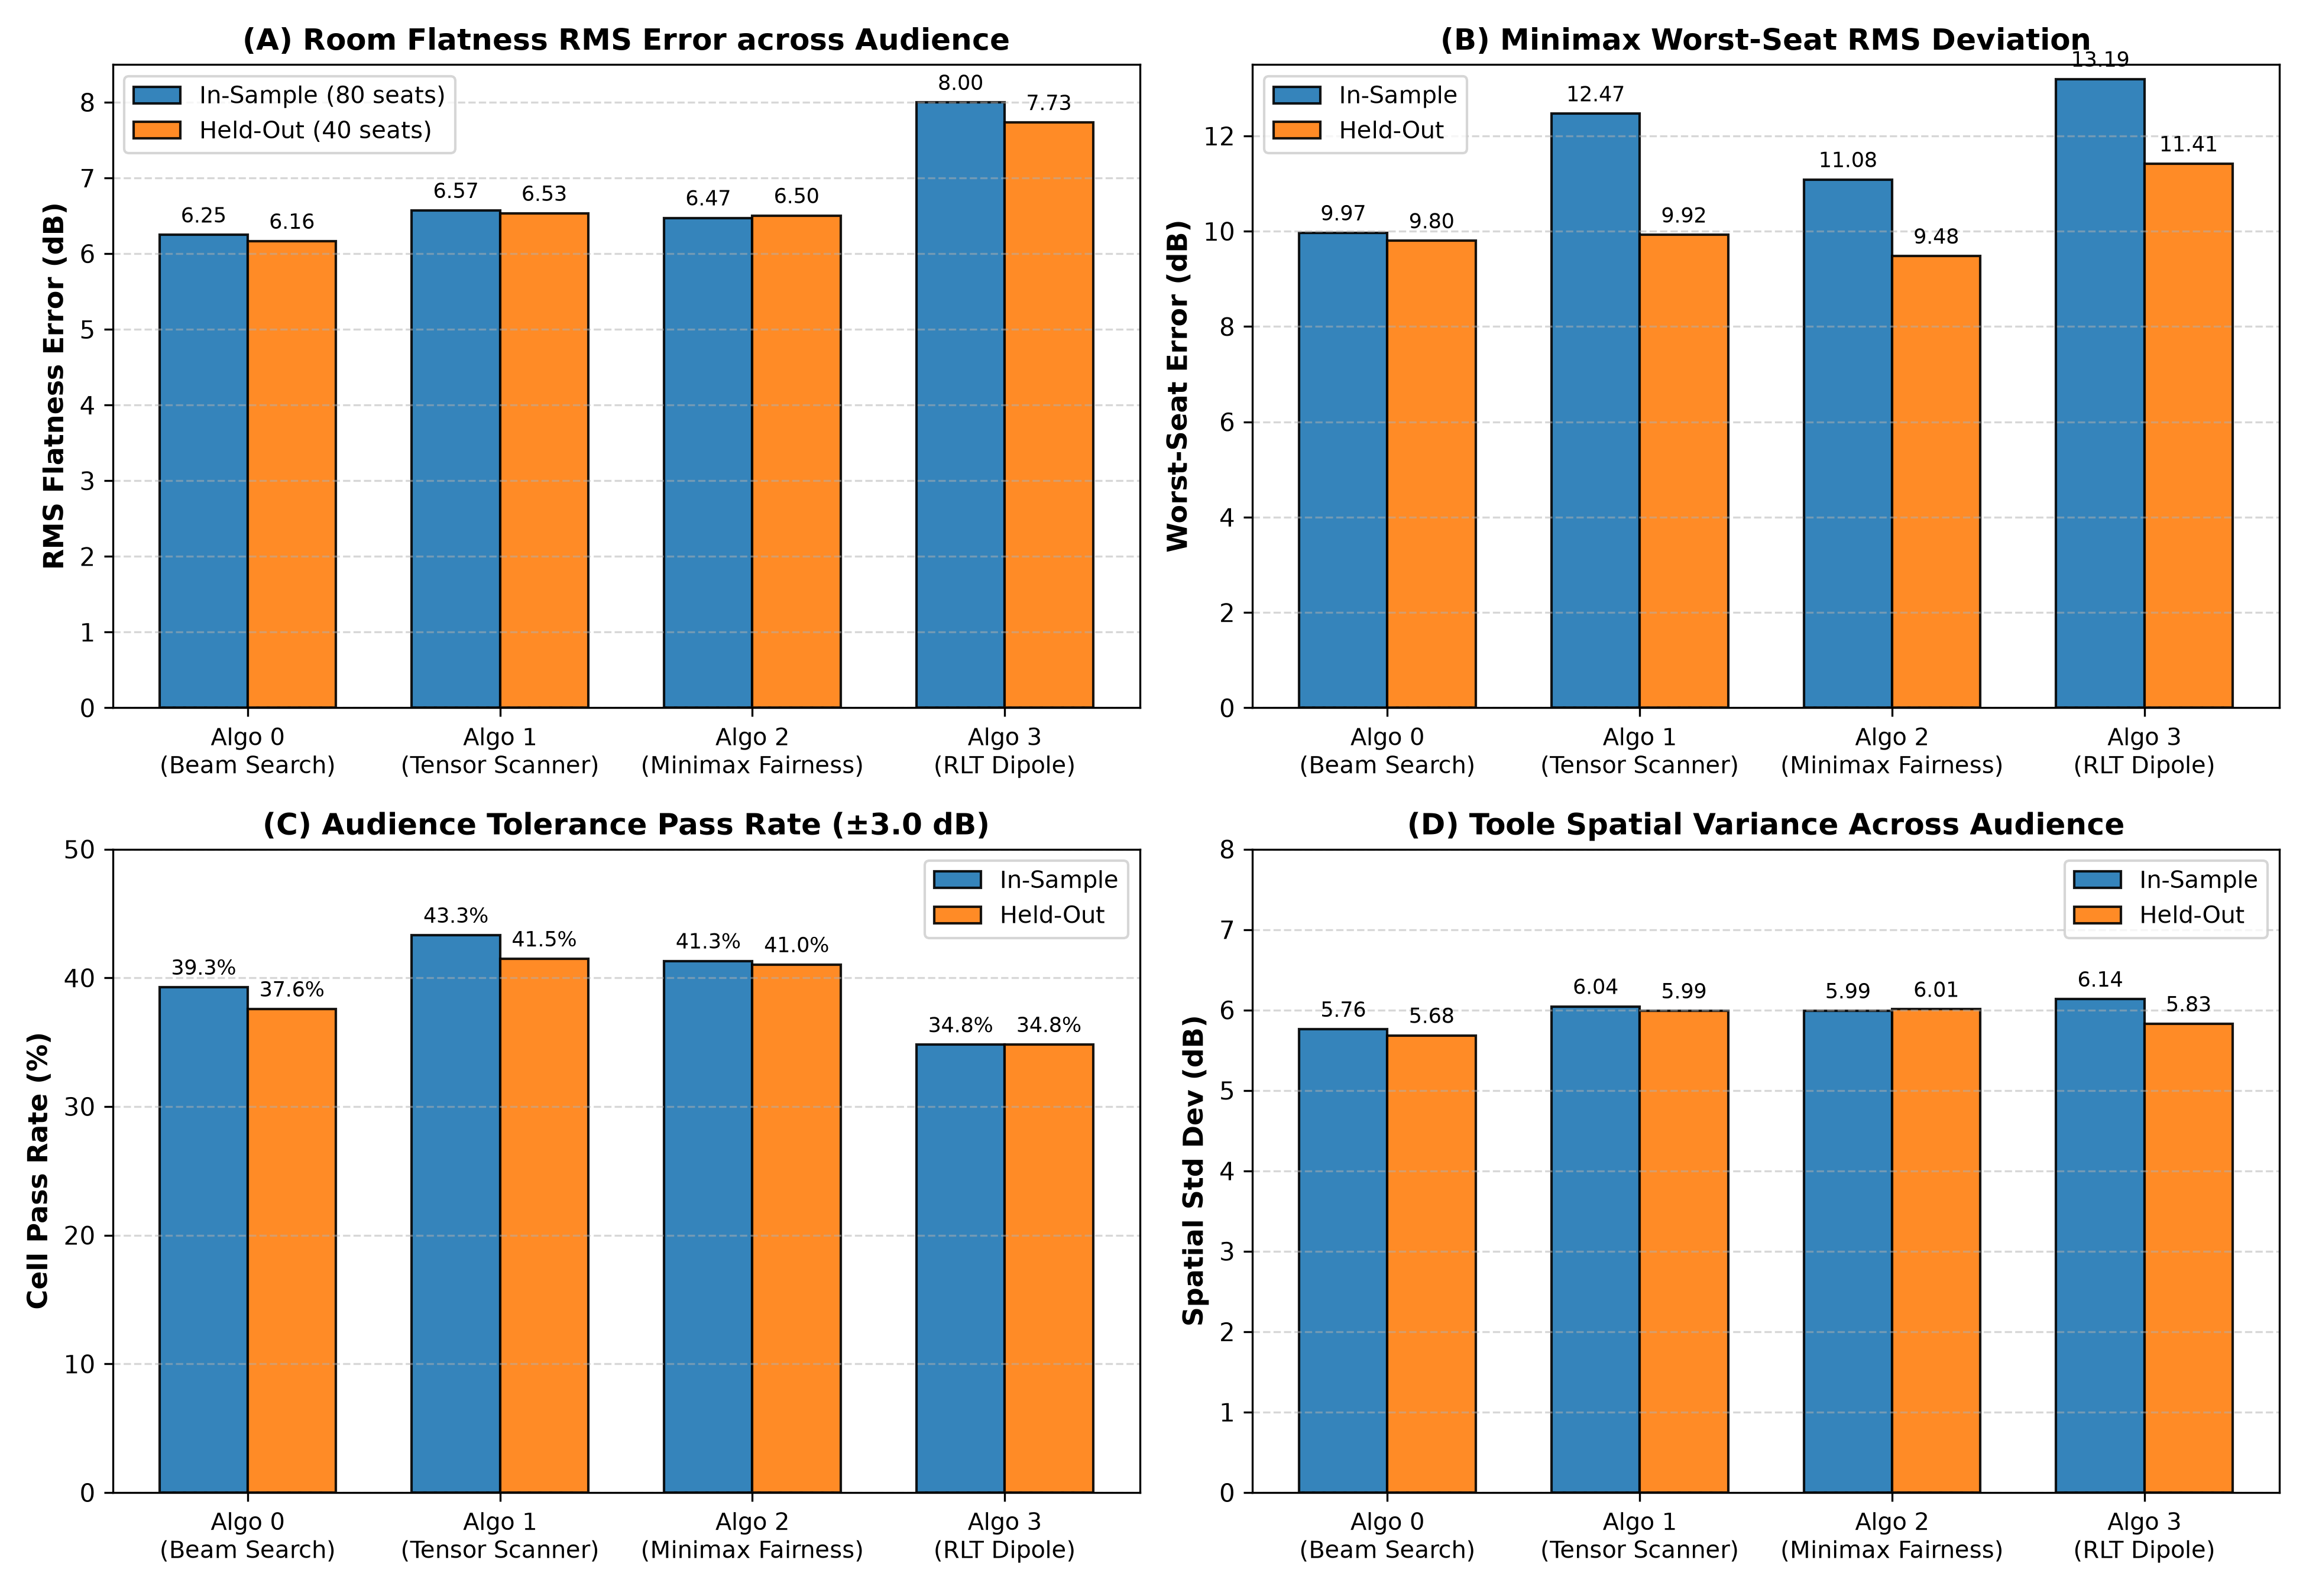
\includegraphics[width=0.92\textwidth]{figures/four_algorithms_comparative_benchmark.png}
\caption{\textbf{Comparative Four-Algorithm Performance Benchmark ($10 \times 12\text{ m}$ Venue).} Panel (A) compares in-sample (80 seats, blue) and held-out (40 off-grid seats, orange) RMS flatness error. Panel (B) presents minimax worst-seat deviation. Panel (C) displays tolerance corridor compliance ($\pm 3.0\text{ dB}$). Panel (D) plots Toole spatial standard deviation across the audience.}
\label{fig:four_algos_benchmark}
\end{figure}

\newpage

\subsection{Continuous 2D Room Acoustic Error Fields Across All Four Algorithms}
Figure~\ref{fig:four_algos_heatmaps} displays the continuous 2D acoustic RMS error field across the entire $10.0 \times 12.0\text{ m}$ hall at ear level ($z = 1.10\text{ m}$), evaluated directly from the exact closed-form modal Green's function without interpolation artifacts.

\begin{figure}[h!]
\centering
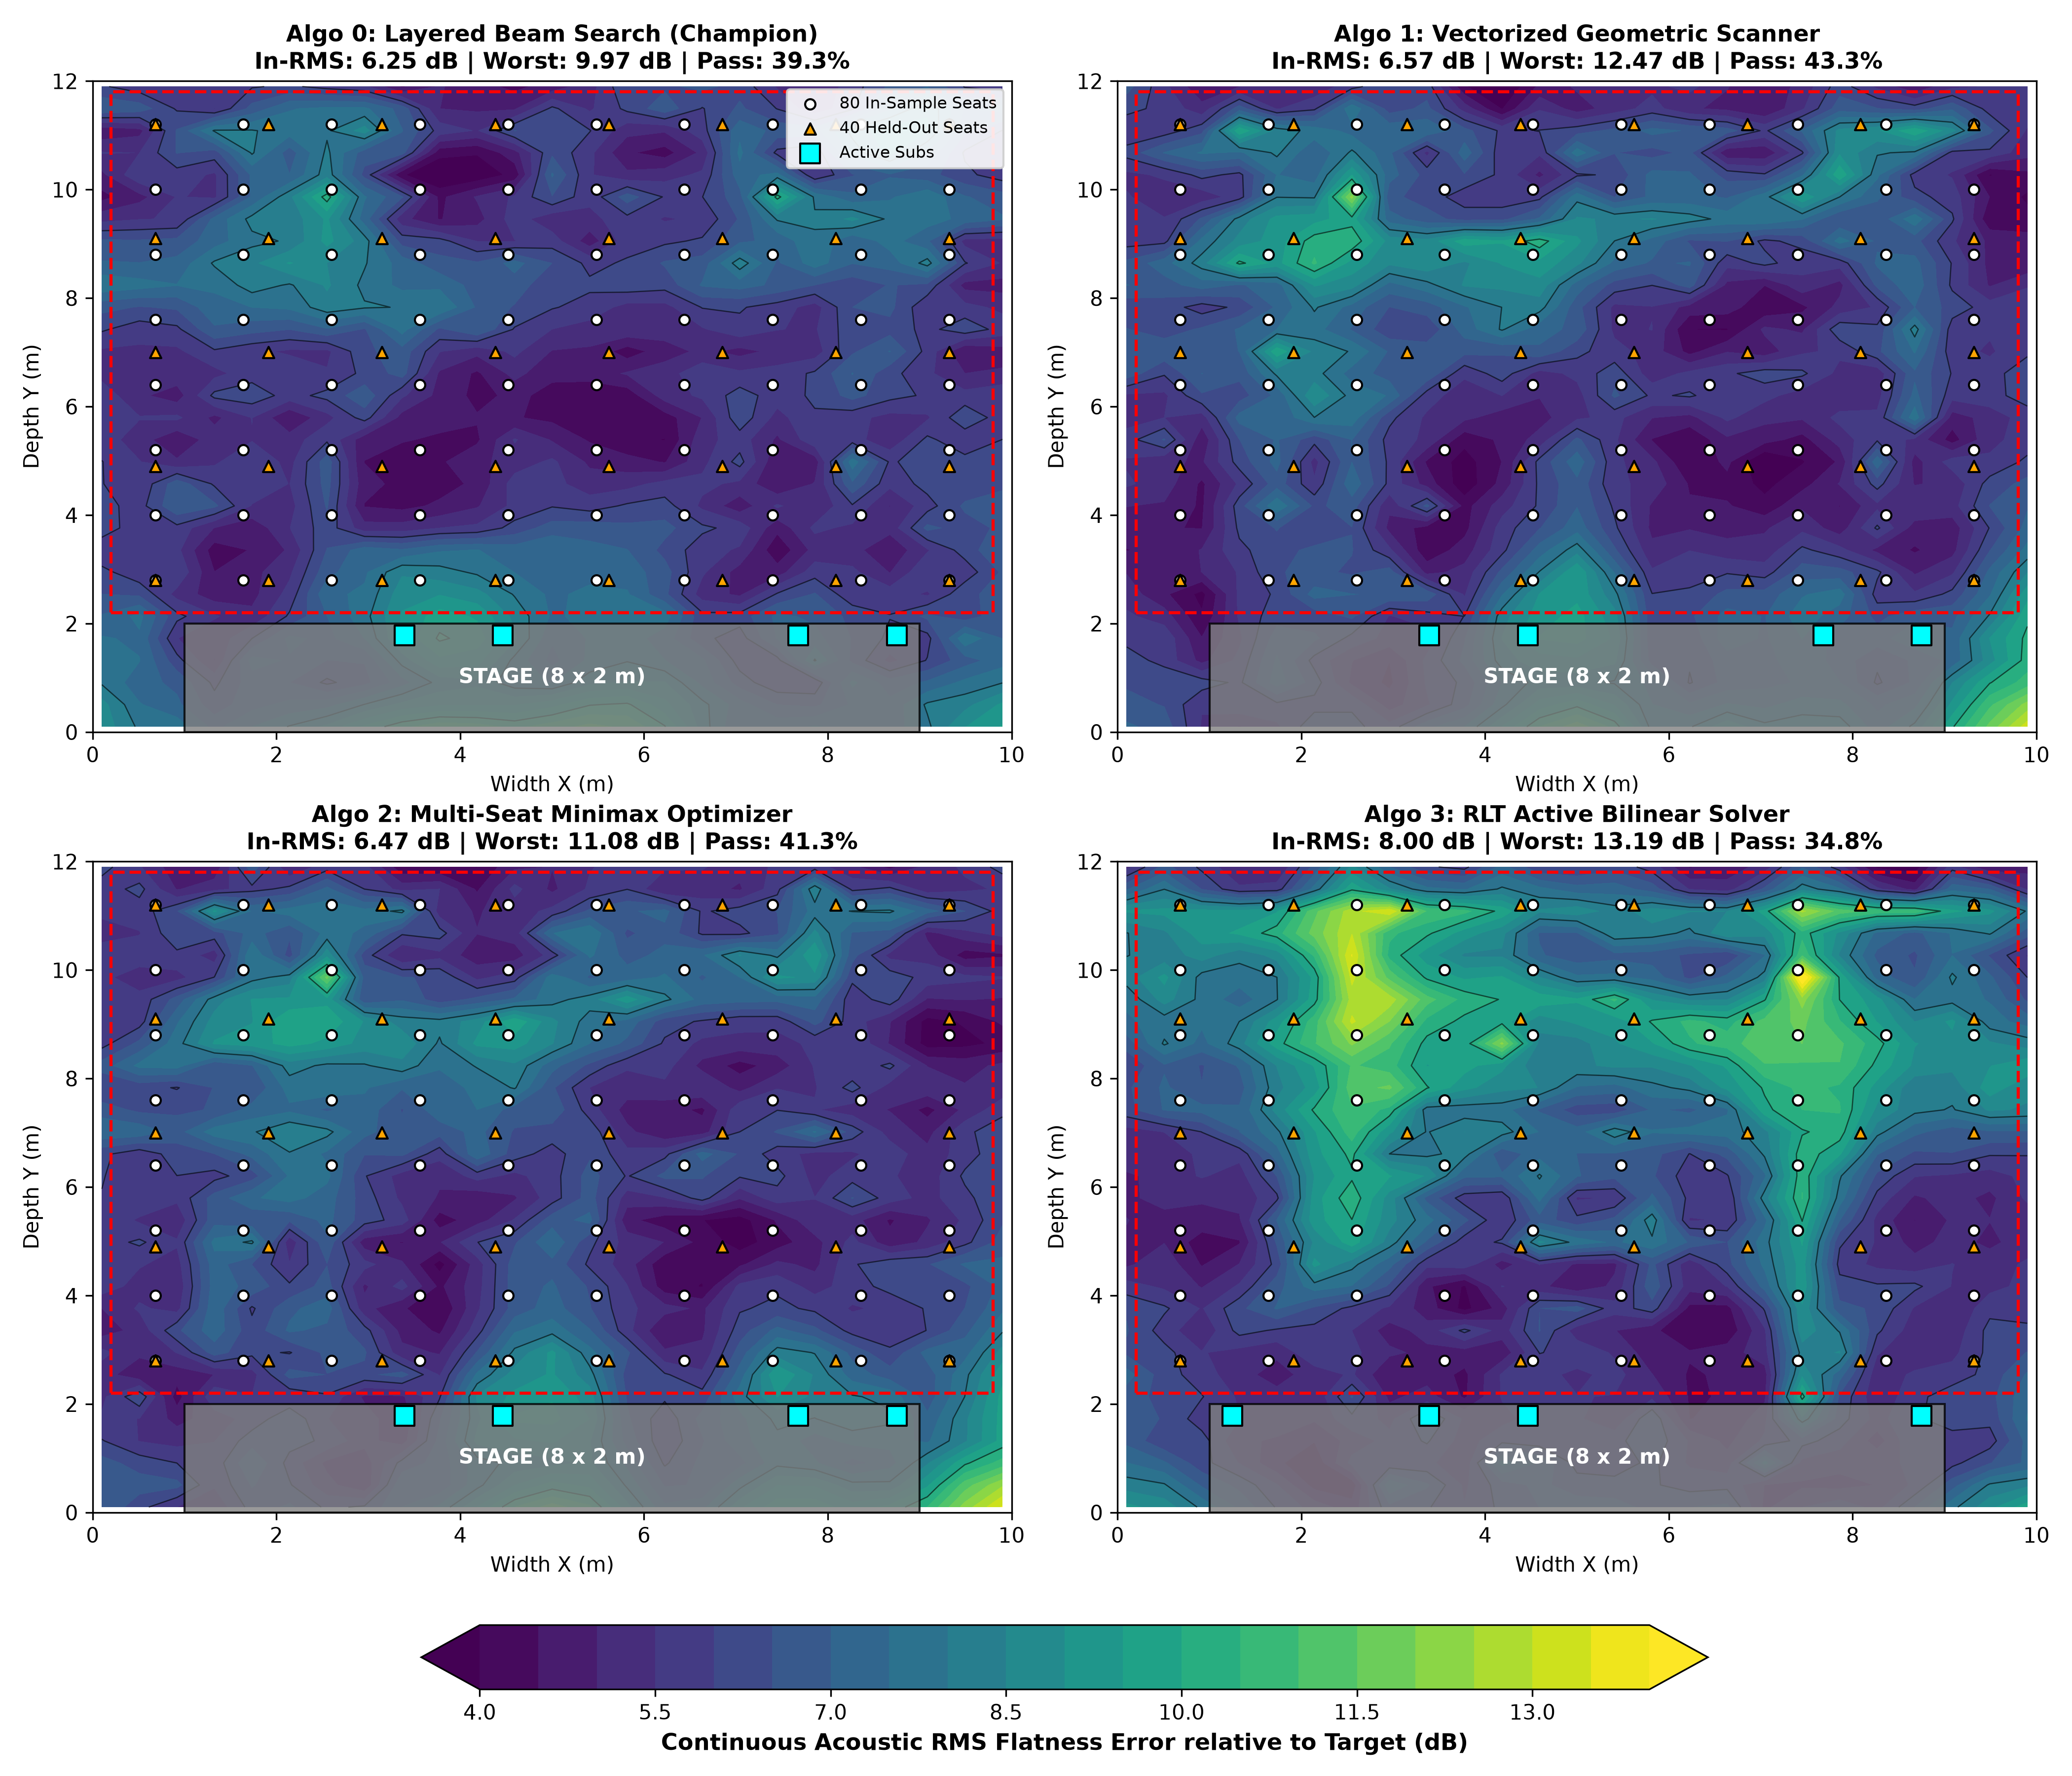
\includegraphics[width=0.92\textwidth]{figures/four_algorithms_acoustic_error_heatmaps.png}
\caption{\textbf{Continuous 2D Acoustic RMS Error Fields for Four Optimization Algorithms.} Contours represent continuous acoustic RMS flatness error relative to target across $20\text{--}200\text{ Hz}$. White circles denote the 80 in-sample seats, orange triangles indicate the 40 held-out off-grid seats, and cyan squares mark active subwoofers along the stage front ($y = 1.78\text{ m}$). The gray rectangle denotes the $8.0 \times 2.0\text{ m}$ centered stage, and the dashed red square denotes the $0.2\text{ m}$ boundary seating margin.}
\label{fig:four_algos_heatmaps}
\end{figure}

\newpage

\subsection{Audience Frequency Response Corridors Across All Four Algorithms}
Figure~\ref{fig:four_algos_corridors} illustrates the individual seat frequency responses across all 80 listener seats, the spatial mean SPL curve, and the $\pm 1\text{ SD}$ spatial variance corridor relative to target $80.0\text{ dB SPL}$.

\begin{figure}[h!]
\centering
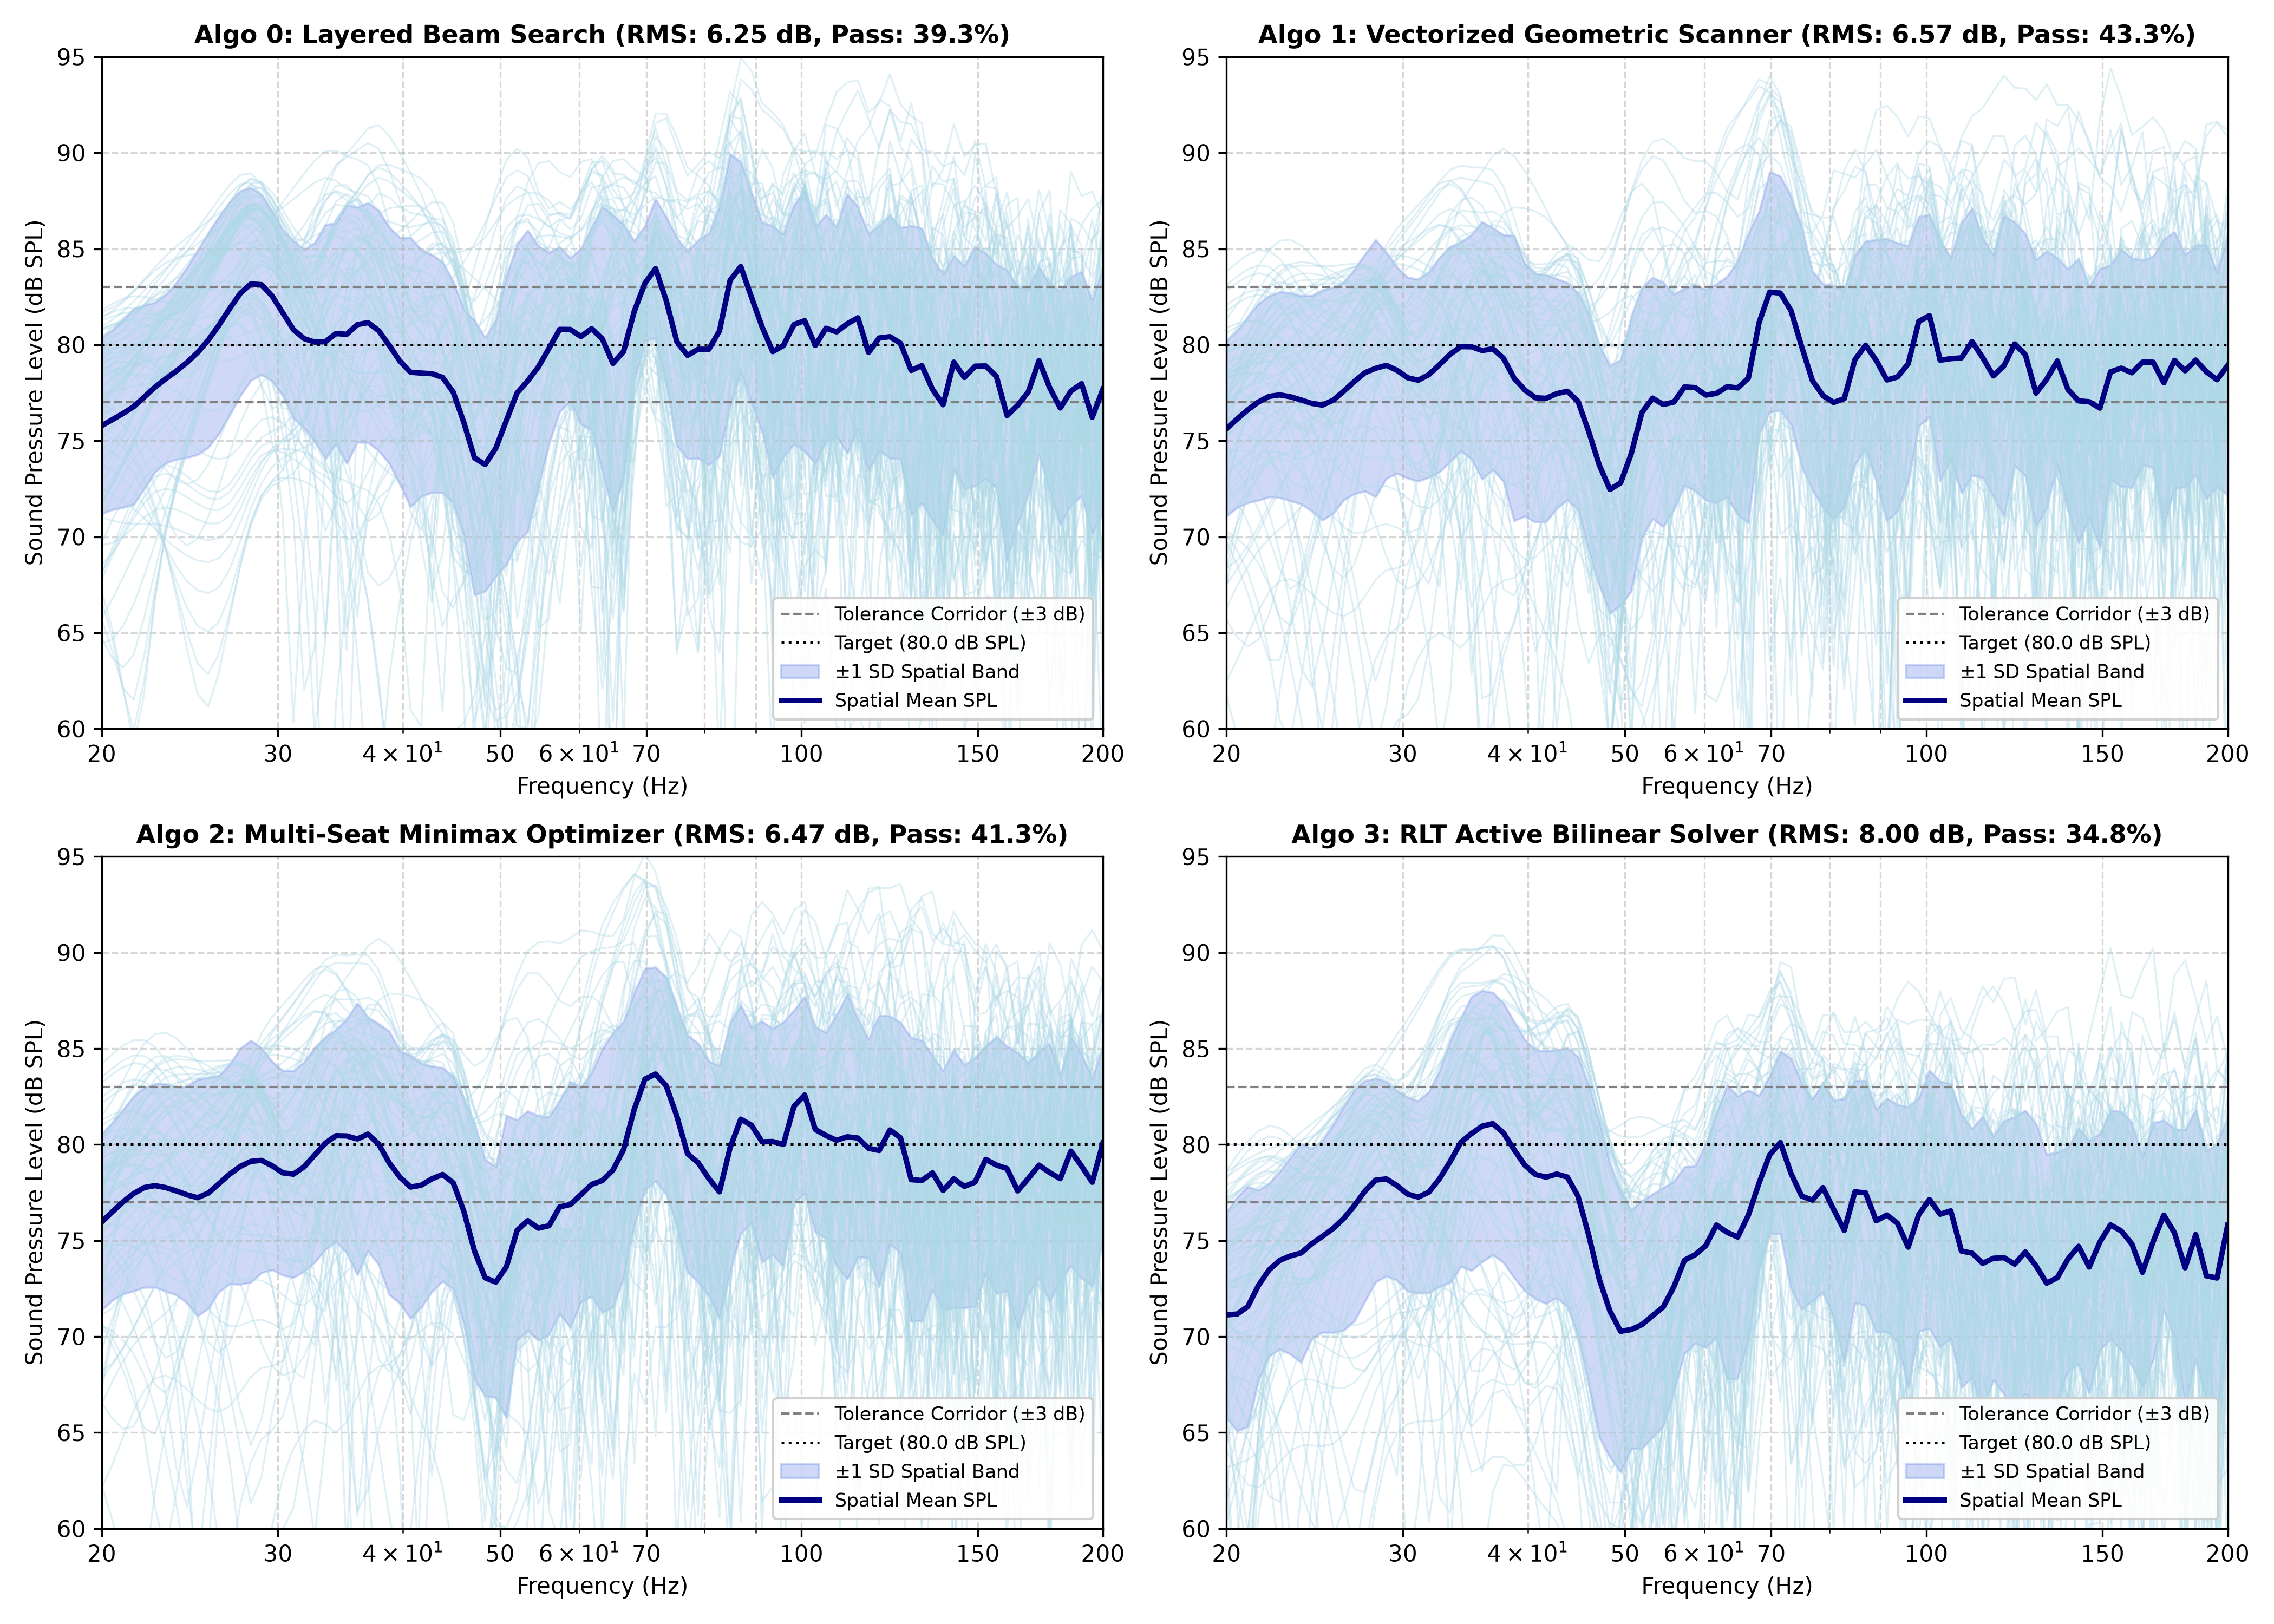
\includegraphics[width=0.92\textwidth]{figures/four_algorithms_frequency_corridors.png}
\caption{\textbf{Audience Frequency Response Corridors Across Four Algorithms ($20\text{--}200\text{ Hz}$).} Light blue curves represent individual seat responses (80 seats). The thick navy curve shows the audience spatial mean SPL, bounded by the $\pm 1\text{ SD}$ shaded envelope and the $\pm 3.0\text{ dB}$ gray dashed tolerance corridor.}
\label{fig:four_algos_corridors}
\end{figure}

\newpage

\subsection{Physical Modal Sound Pressure Field Slices}
Figure~\ref{fig:four_algos_modal_slices} presents continuous spatial sound pressure level slices across the room at four characteristic frequencies ($20.0\text{ Hz}, 50.0\text{ Hz}, 100.0\text{ Hz}, 200.0\text{ Hz}$).

\begin{figure}[h!]
\centering
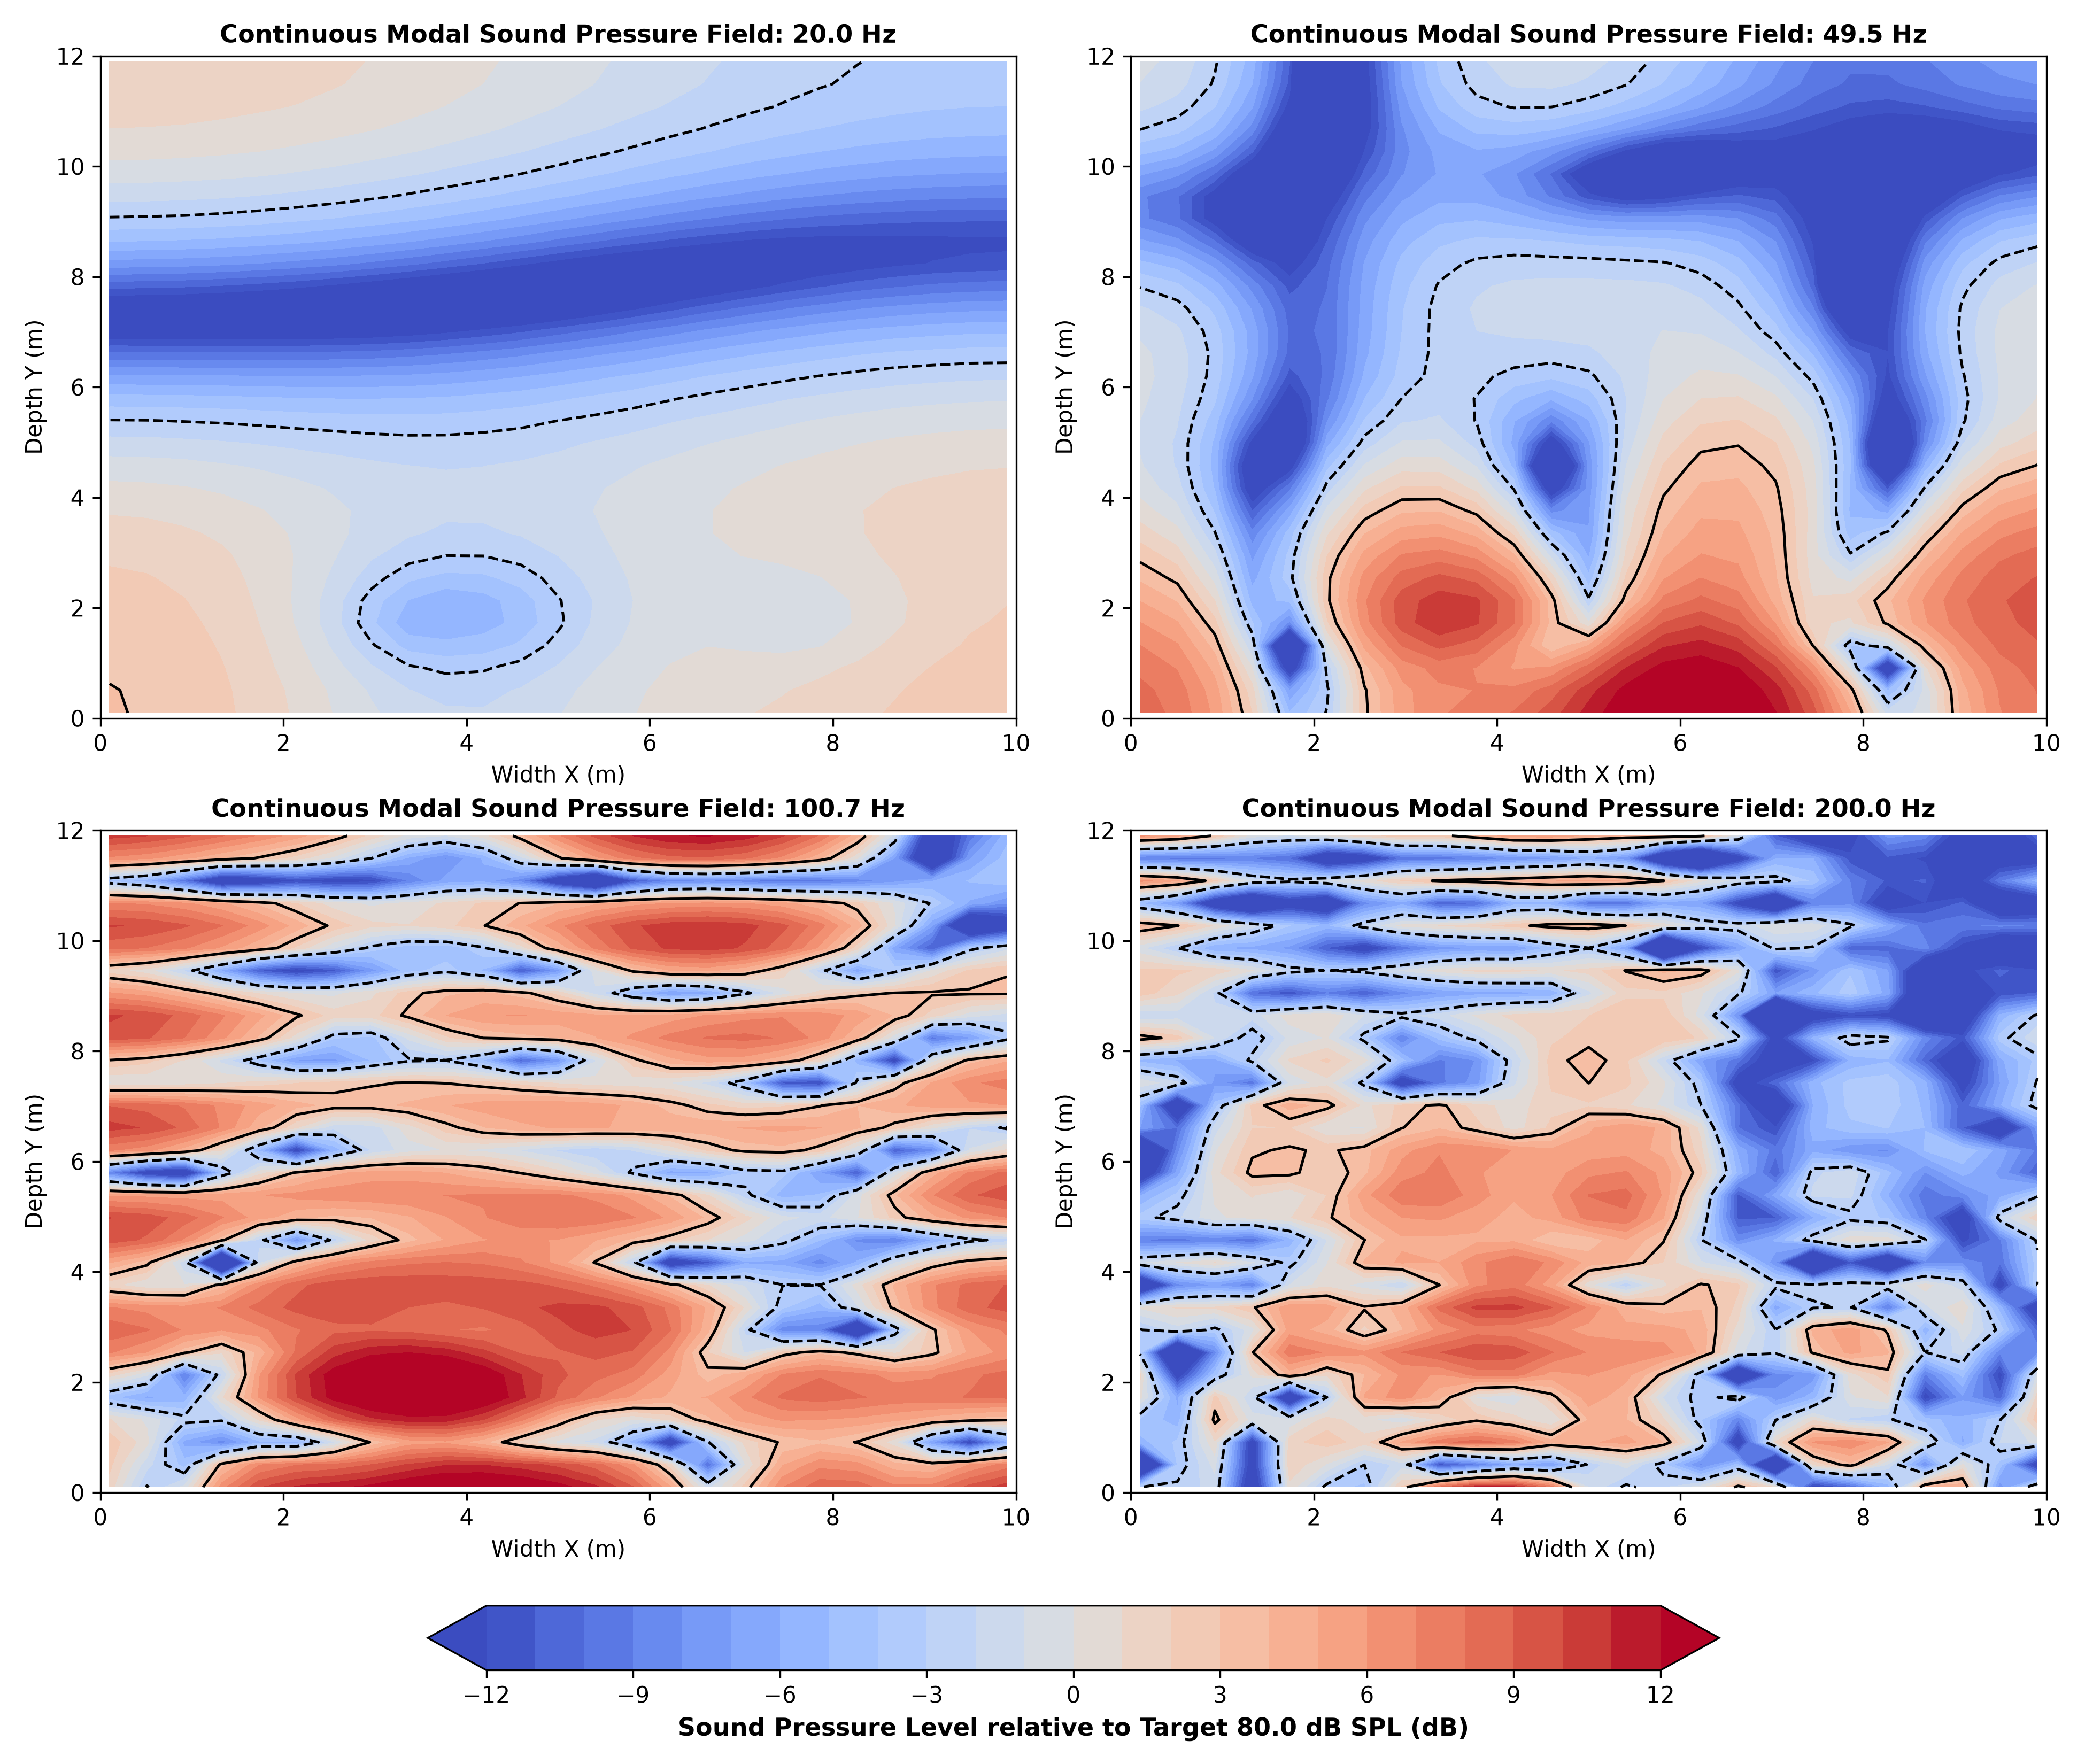
\includegraphics[width=0.88\textwidth]{figures/four_algorithms_modal_slices.png}
\caption{\textbf{Physical Modal Sound Pressure Field Slices across the Venue.} Color contours show sound pressure level in dB relative to $80.0\text{ dB SPL}$. Solid black contours denote the $\pm 3.0\text{ dB}$ tolerance boundaries. At $20.0\text{ Hz}$, an interference null band forms across $y \approx 7.5\text{ m}$. At $50.0\text{ Hz}$, transverse and longitudinal modes interact. At $100.0\text{ and }200.0\text{ Hz}$, dense multimodal wave interference patterns emerge above the Schroeder cutoff ($f_s \approx 73.2\text{ Hz}$).}
\label{fig:four_algos_modal_slices}
\end{figure}

\newpage

\subsection{Audience Conjunction Spectrum and Passing-Tone Distributions}
Figures~\ref{fig:four_algos_conjunction} and~\ref{fig:four_algos_histograms} present audience fairness diagnostics, including the audience conjunction spectrum $N(k)$ and individual seat passing-tone histograms.

\begin{figure}[h!]
\centering
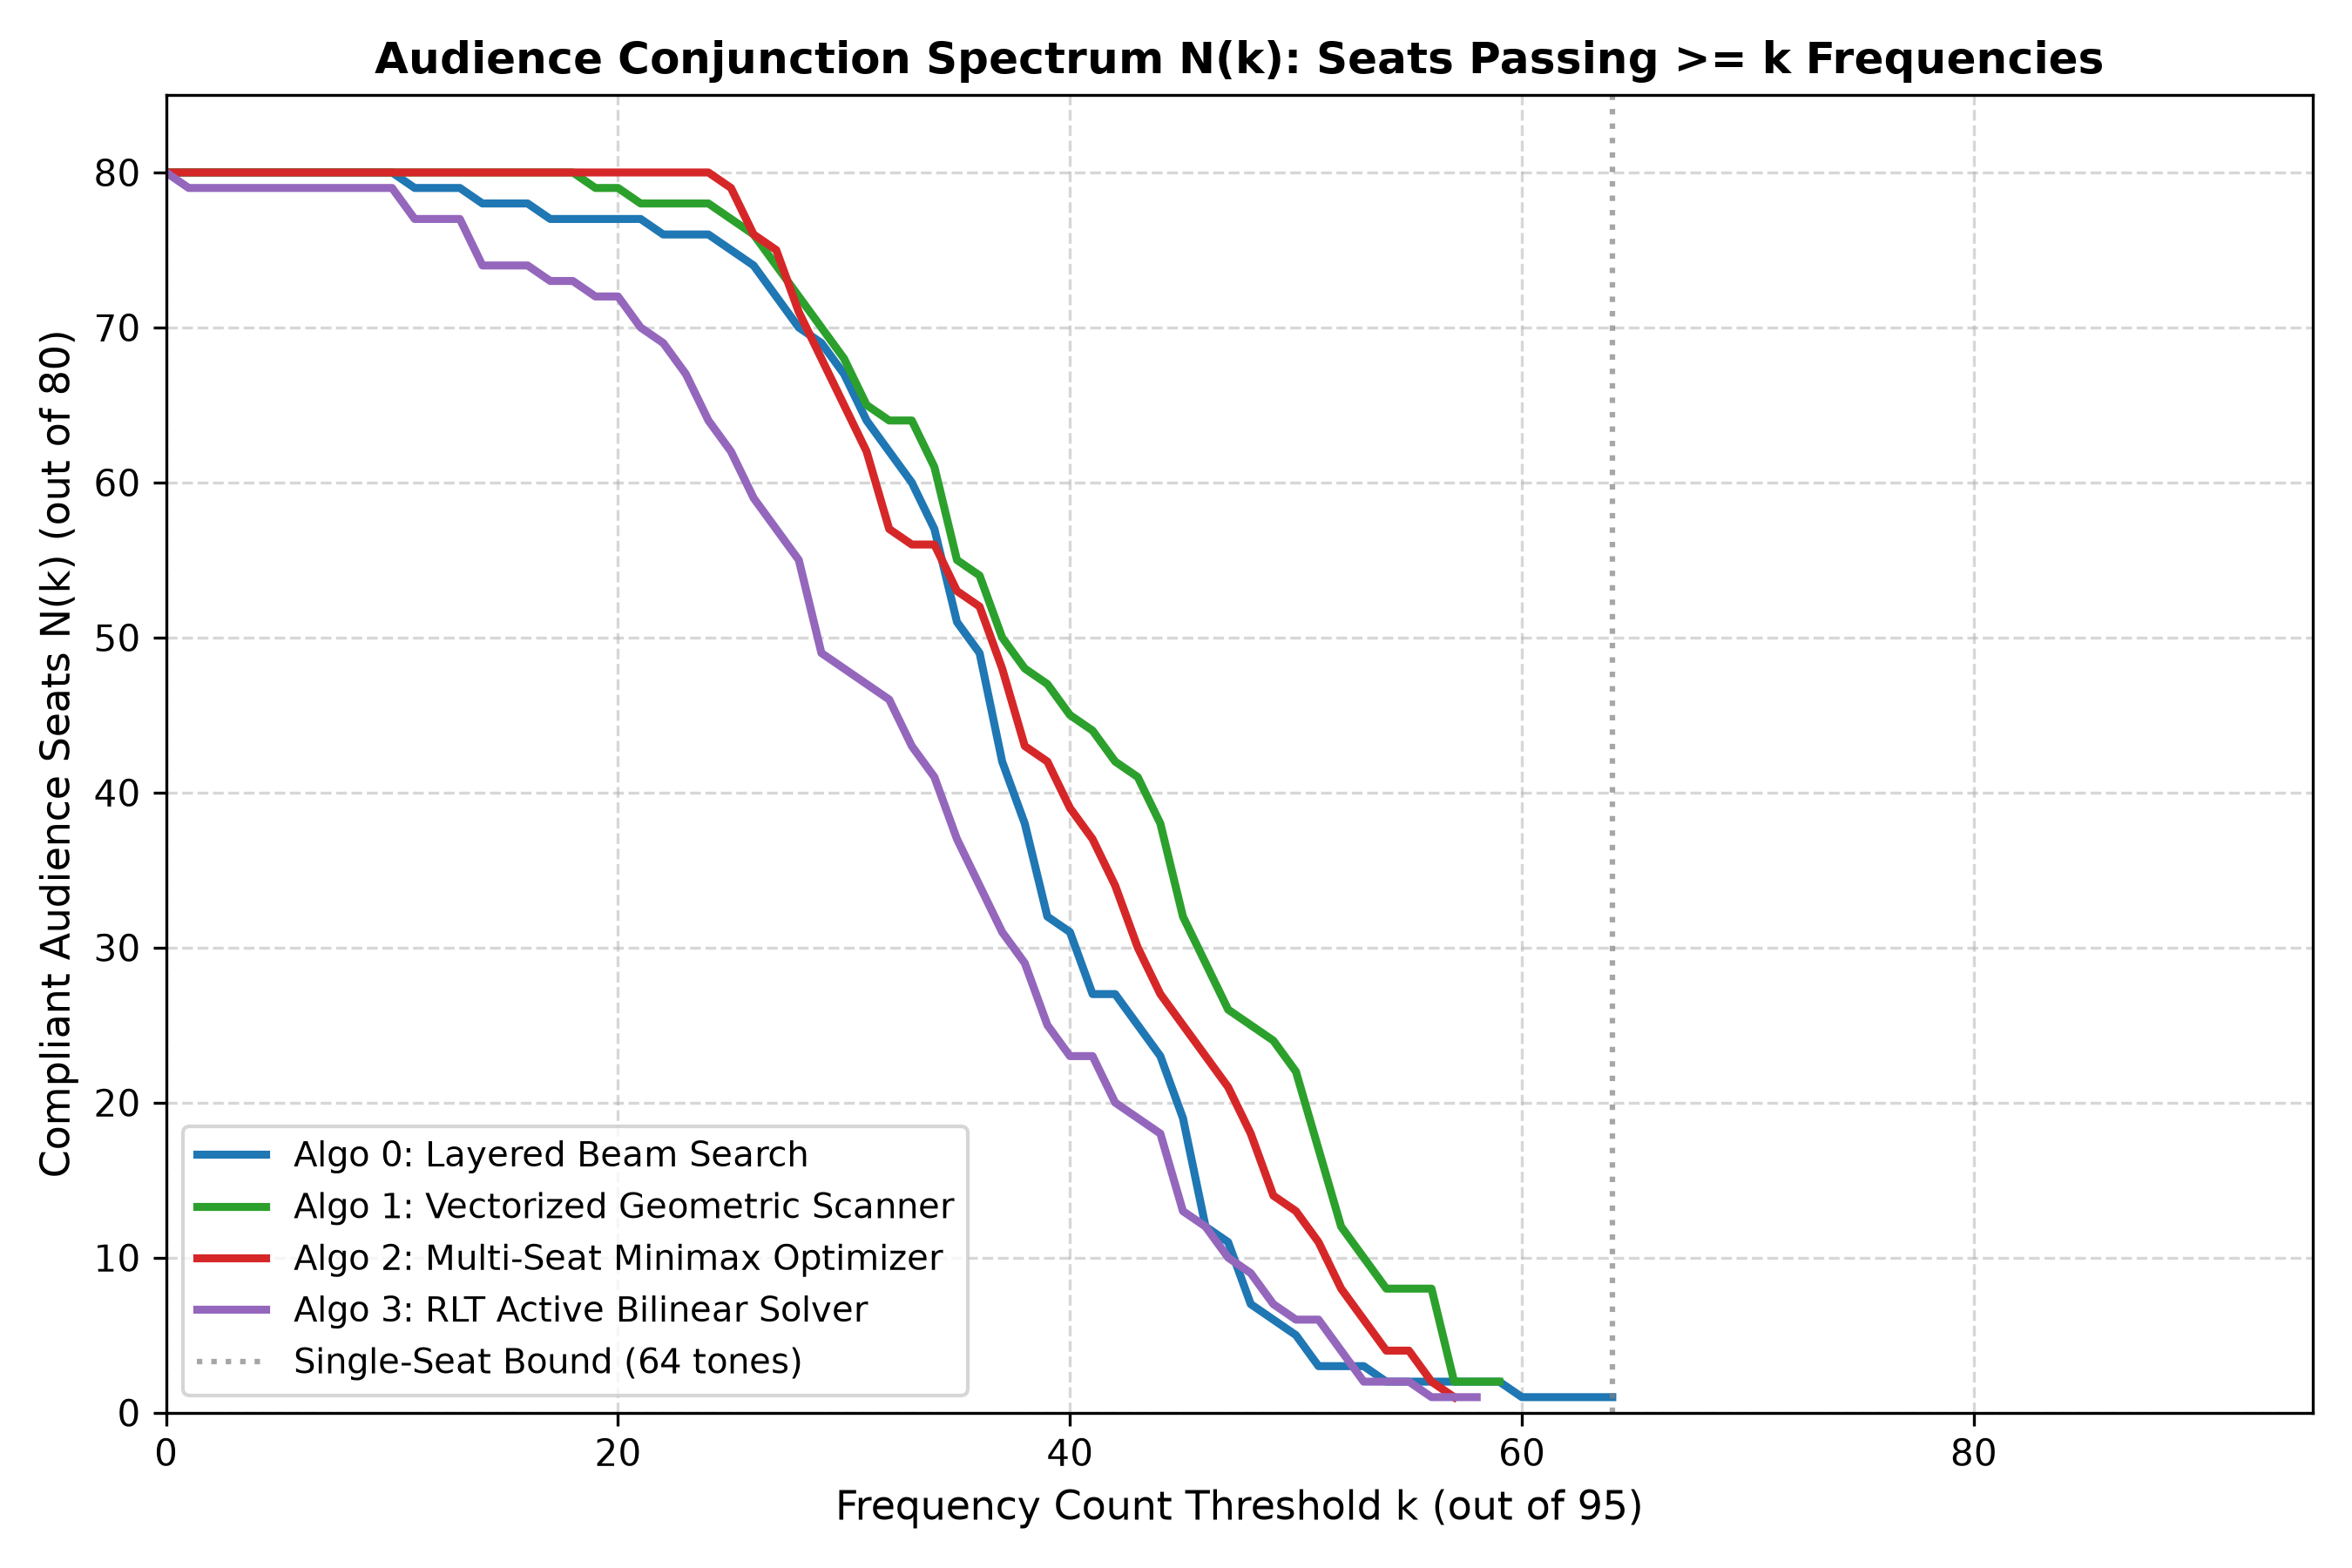
\includegraphics[width=0.86\textwidth]{figures/four_algorithms_conjunction_spectrum.png}
\caption{\textbf{Audience Conjunction Spectrum $N(k)$ Across Four Algorithms.} Curves show the number of audience seats $N(k)$ that simultaneously pass at least $k$ frequencies. Notice Algorithm 2 guarantees $N(24) = 80$ (100\% of seats pass at least 24 tones), whereas Algorithm 0 drops below 80 seats at $k = 11$, and Algorithm 3 has seats with 0 passing tones.}
\label{fig:four_algos_conjunction}
\end{figure}

\begin{figure}[h!]
\centering
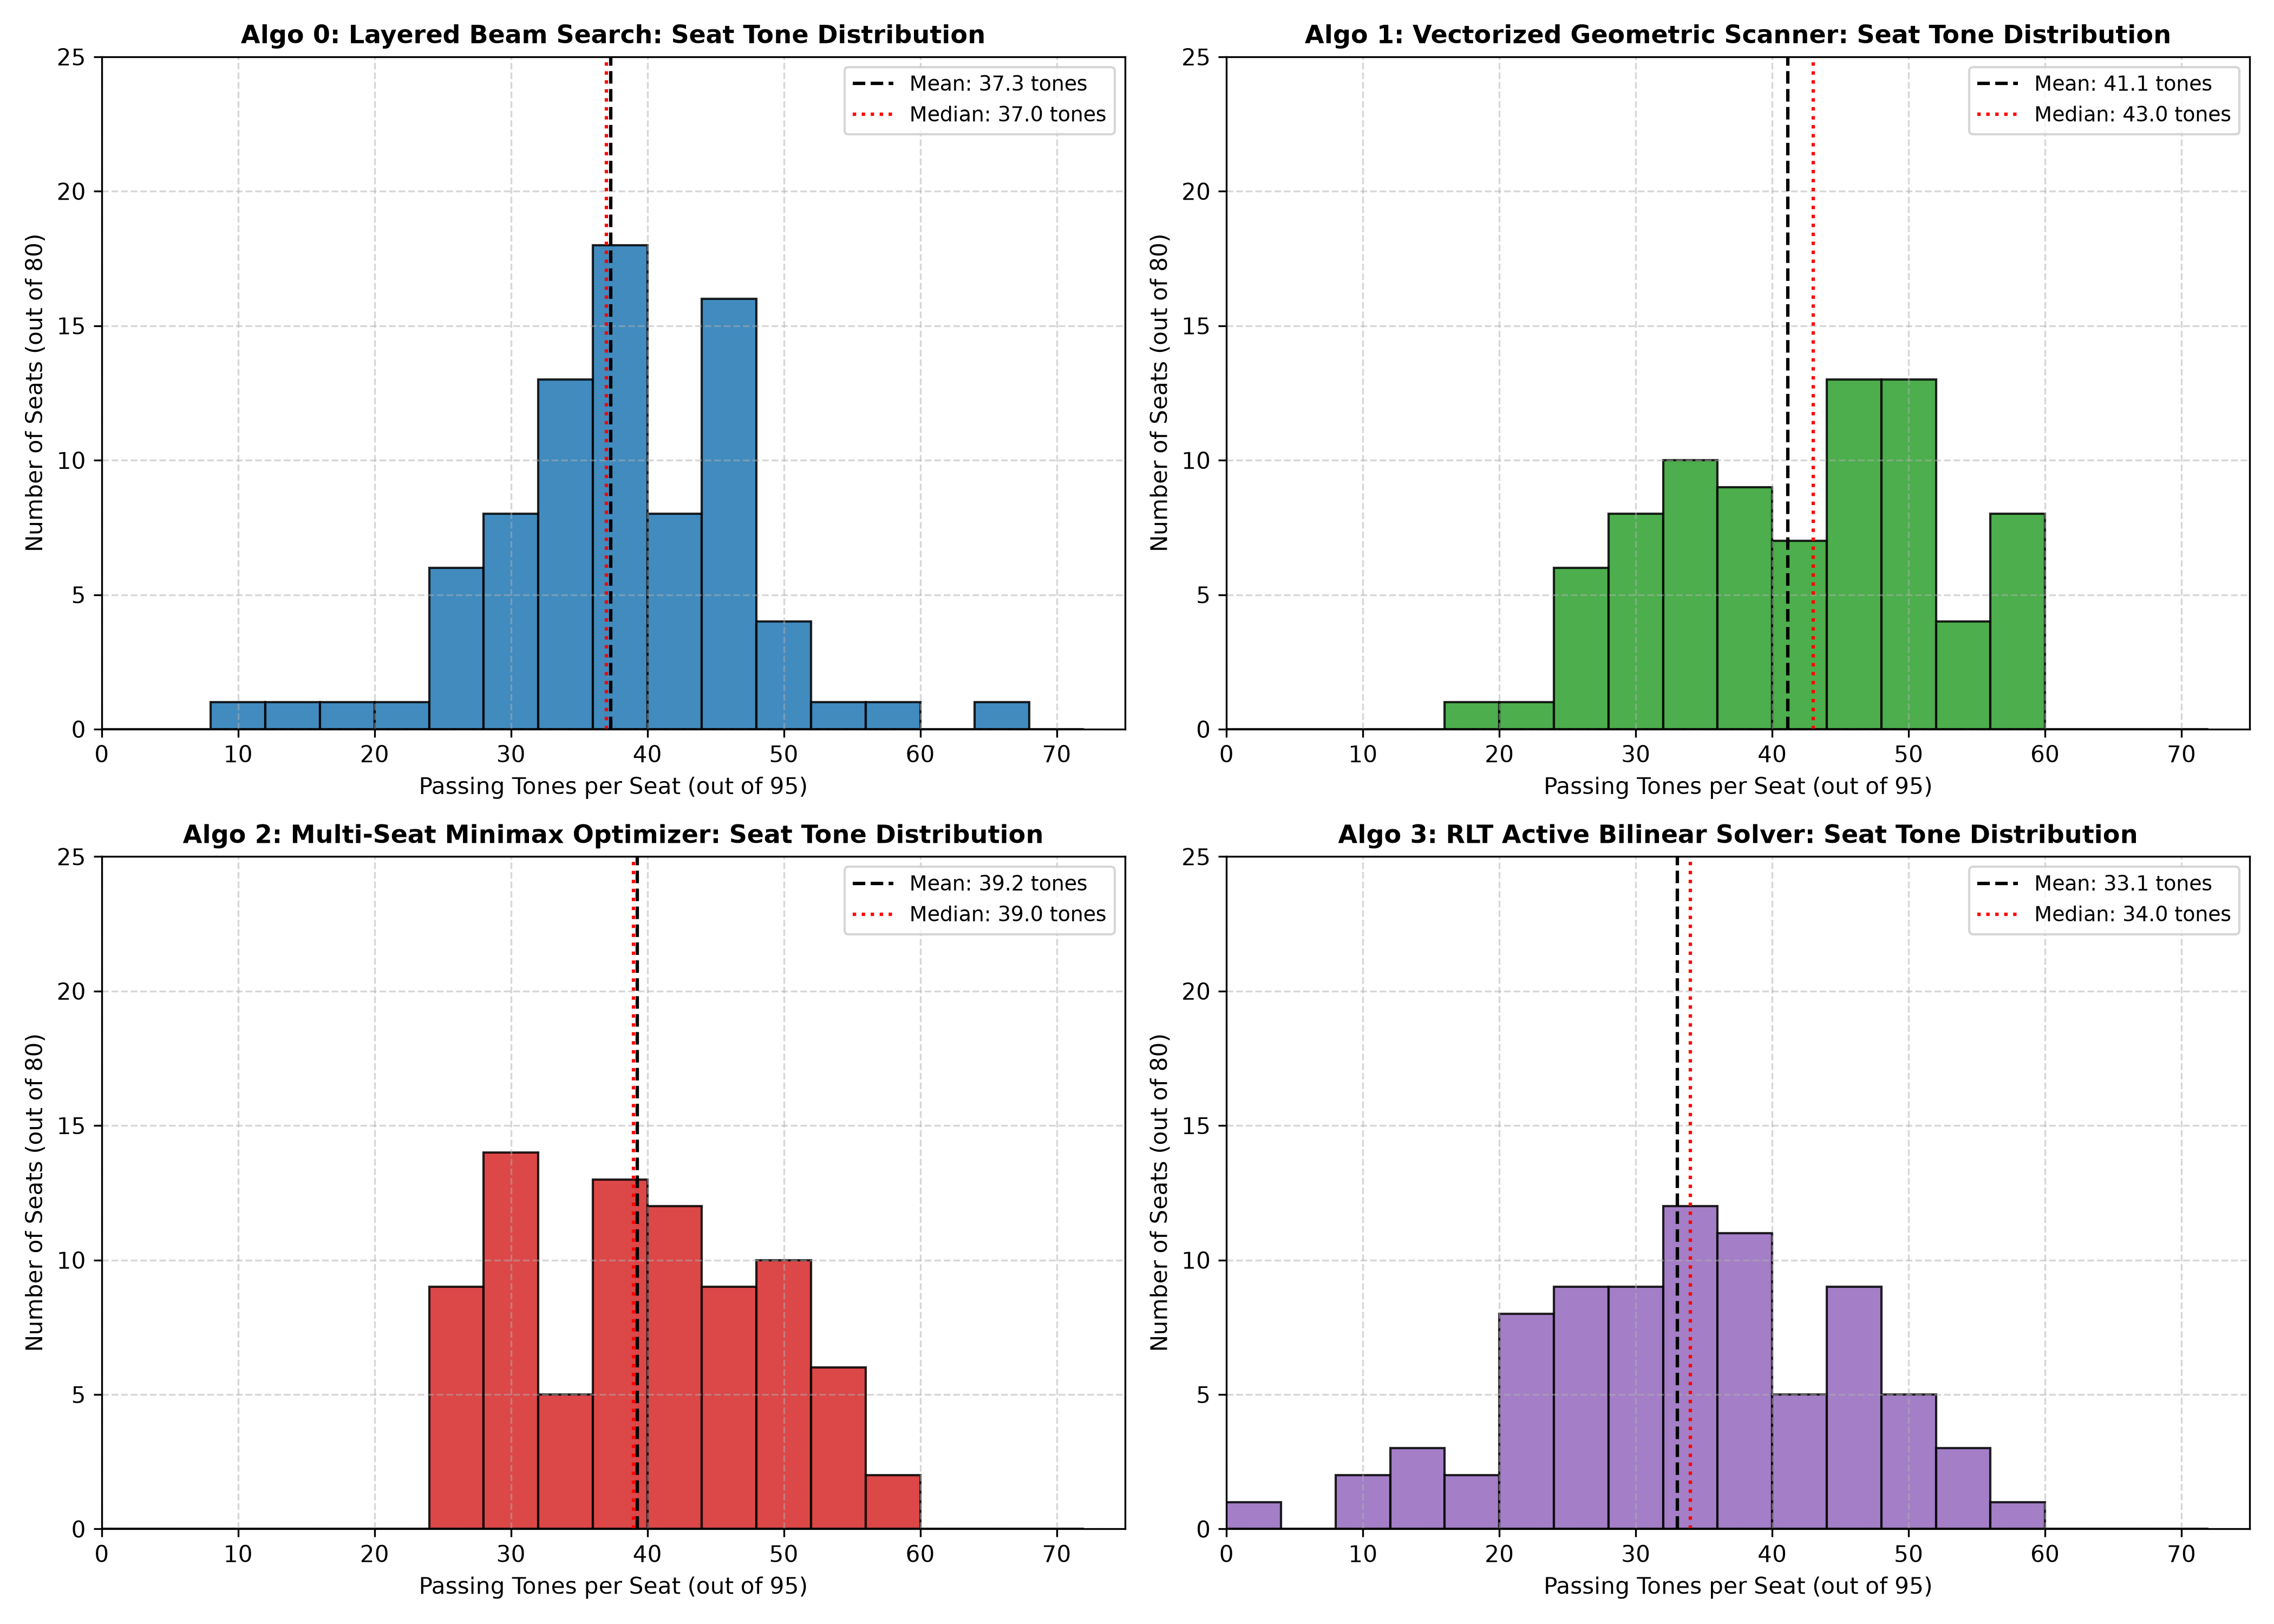
\includegraphics[width=0.90\textwidth]{figures/four_algorithms_seat_histograms.png}
\caption{\textbf{Audience Seat Passing-Tone Histograms Across Four Algorithms.} Histograms show the distribution of compliant tones per seat across all 80 audience positions. Black dashed line marks the audience mean; red dotted line marks the audience median.}
\label{fig:four_algos_histograms}
\end{figure}

\newpage

\subsection{Environmental and Physical Tolerance Sensitivity}
Figure~\ref{fig:monte_carlo} presents the 256-realization physical Monte Carlo analysis evaluating the stability of the optimized front-stage array under environmental perturbations.

\begin{figure}[h!]
\centering
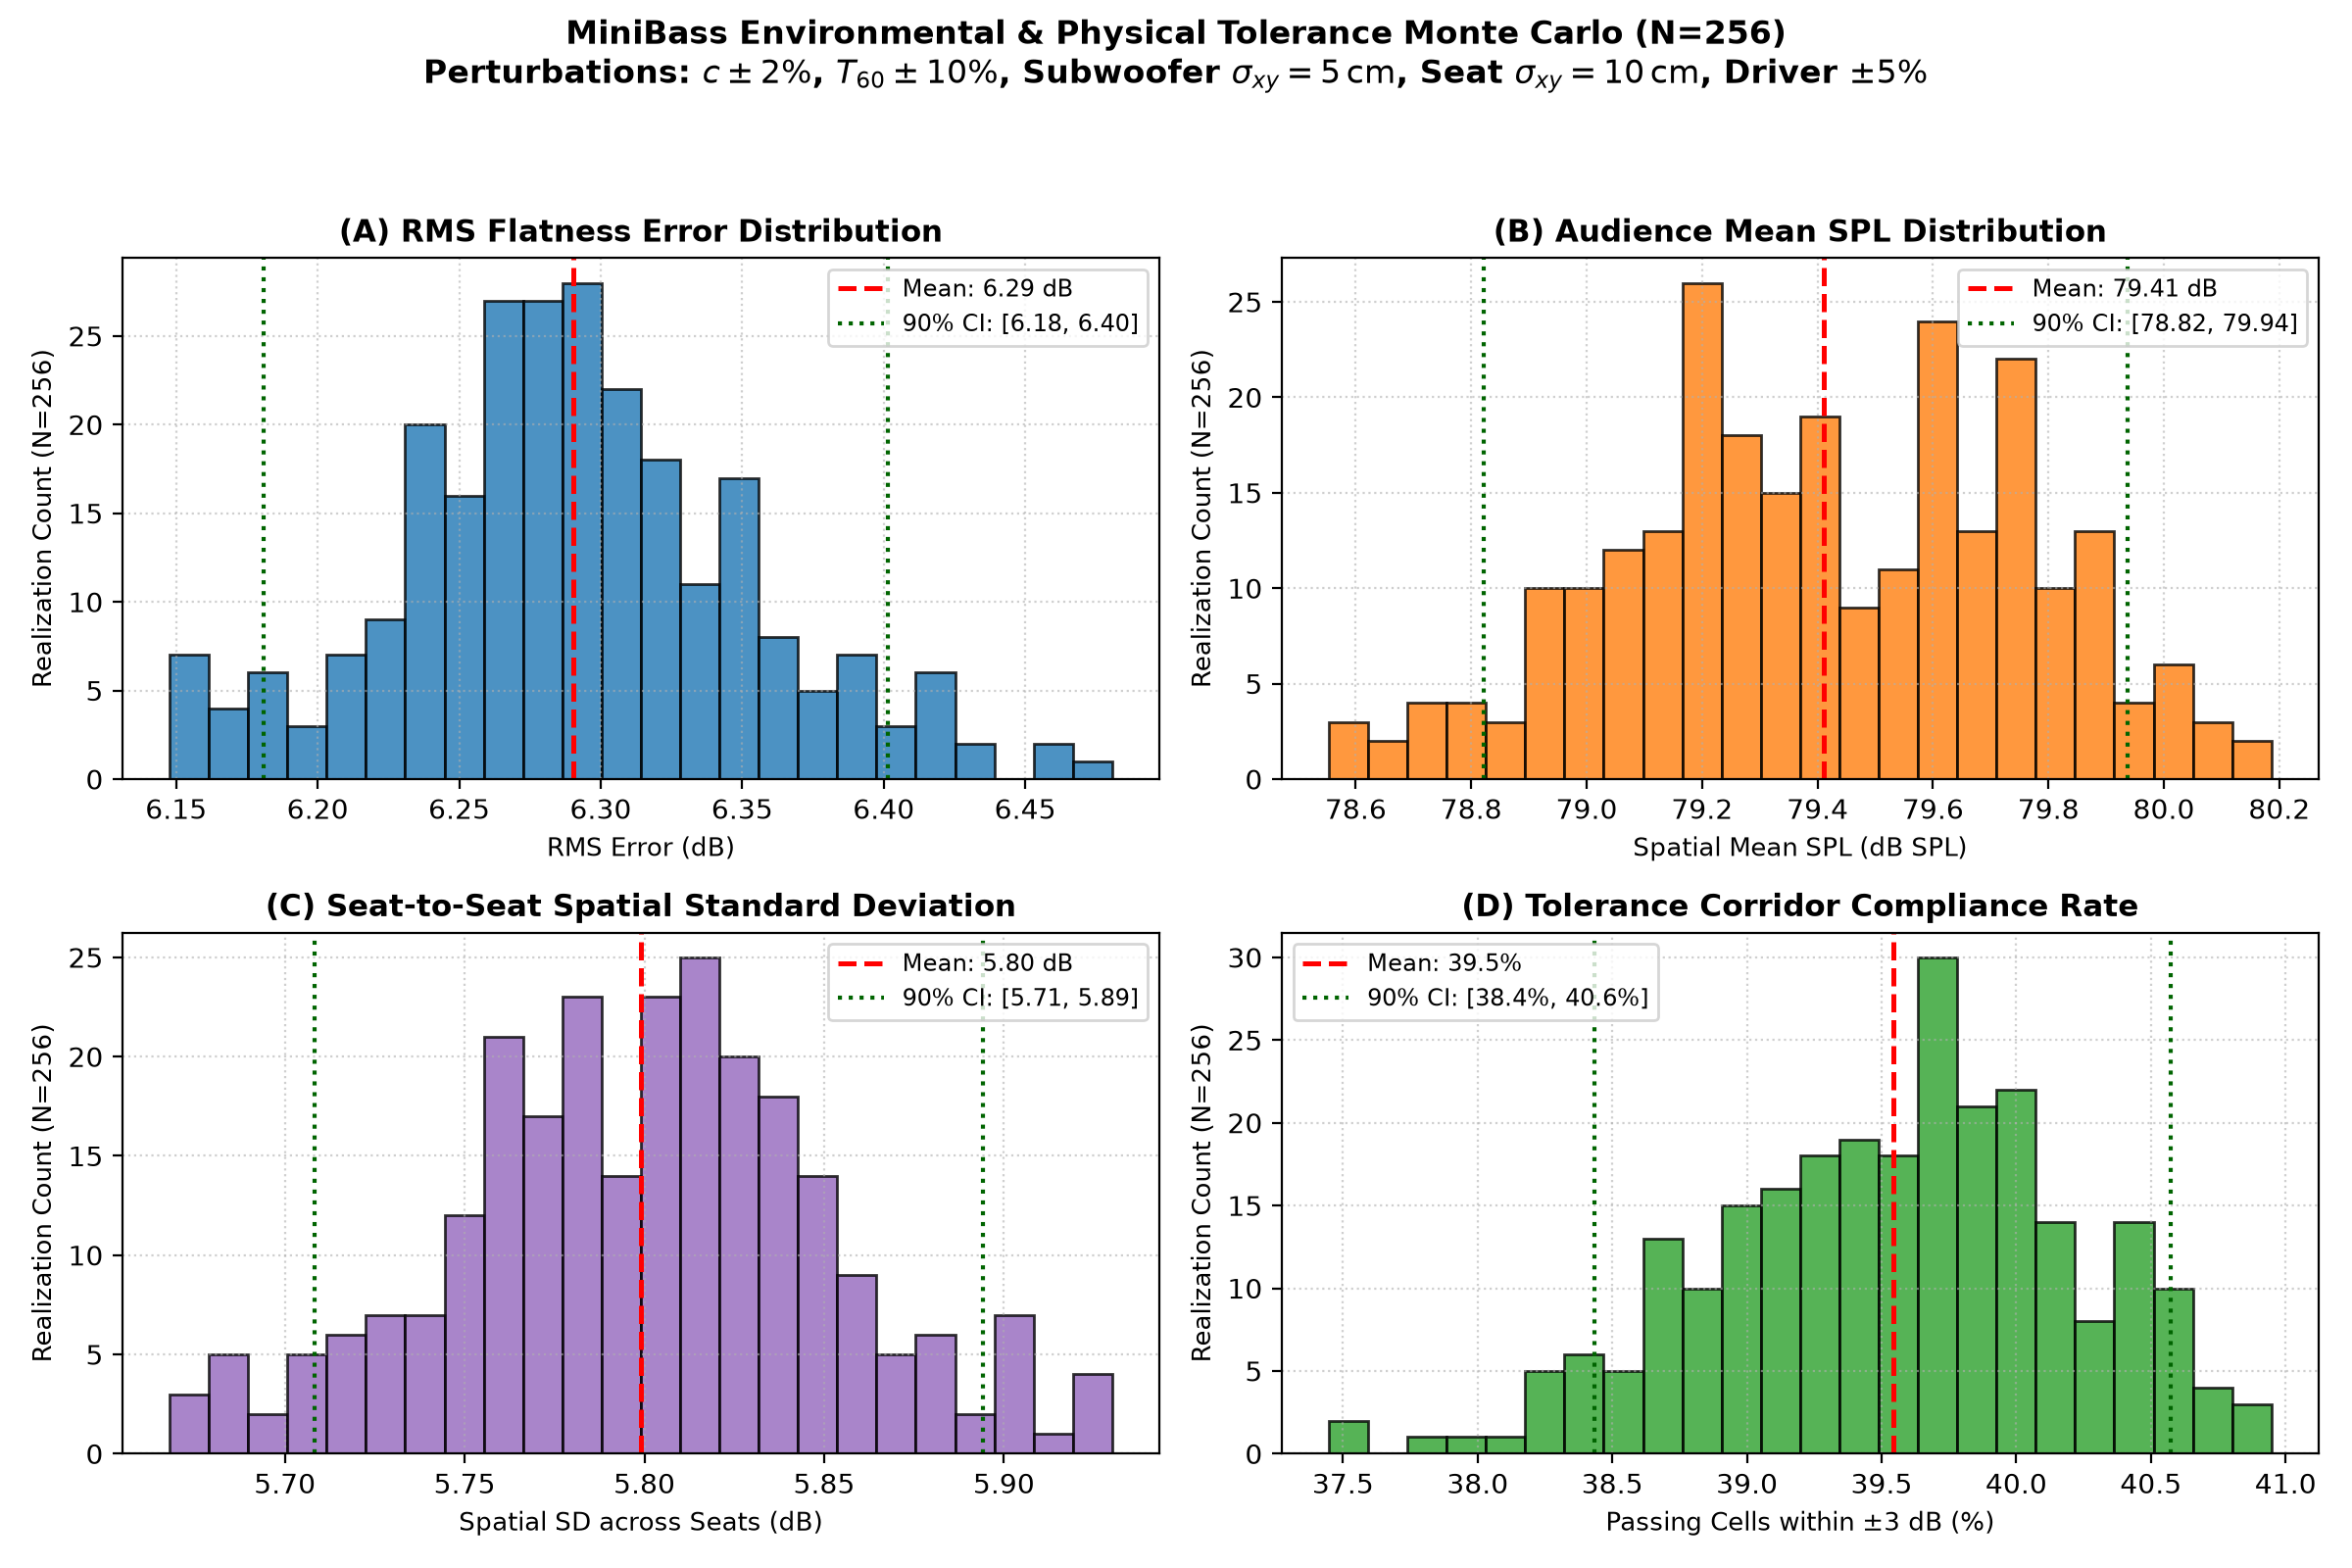
\includegraphics[width=0.88\textwidth]{figures/dryrun_10x12_physical_monte_carlo.png}
\caption{\textbf{Environmental and Physical Tolerance Monte Carlo (256 Realizations).} Realizations perturb sound speed $c \pm 2\%$, reverberation time $T_{60} \pm 10\%$, subwoofer placement $\sigma_{xy} = 5\text{ cm}$, seat coordinates $\sigma_{xy} = 10\text{ cm}$, and driver parameters $\pm 5\%$. Panel (A) shows the RMS error distribution (mean $6.29\text{ dB}$, 90\% CI $[6.18, 6.40]\text{ dB}$). Panel (B) shows spatial mean SPL. Panel (C) displays seat-to-seat spatial standard deviation. Panel (D) presents tolerance corridor compliance.}
\label{fig:monte_carlo}
\end{figure}

\newpage

% ==============================================================================
% SECTION 5: PRACTICAL GUIDELINES & SELECTION MATRIX
% ==============================================================================
\section{Practical Algorithmic Selection Guide and Engineering Rules}

\subsection{Algorithmic Selection Matrix}
Based on empirical findings across the $10 \times 12\text{ m}$ venue, Table~\ref{tab:selection_matrix} provides a practical engineering decision guide for selecting an optimization algorithm based on venue requirements.

\begin{table}[h!]
\centering
\small
\renewcommand{\arraystretch}{1.3}
\caption{Algorithmic Selection Matrix for Multi-Subwoofer Venue Synthesis}
\label{tab:selection_matrix}
\begin{tabularx}{\textwidth}{|p{4.6cm}|p{4.2cm}|X|}
\hline
\textbf{Target Operational Scenario} & \textbf{Recommended Algorithm} & \textbf{Engineering Justification} \\ \hline
\textbf{Reference Recording Studio / Critical Mastering Suite} & \textbf{Algorithm 0} \newline (Layered Beam Search) & Minimizes quadratic $L_2$ error ($6.25\text{ dB}$ RMS), providing the most neutral total energy response across seats. \\ \hline
\textbf{Commercial Cinema / Auditorium Acceptance Testing} & \textbf{Algorithm 1} \newline (Geometric Tensor Scanner) & Directly maximizes tolerance corridor cell compliance ($43.3\%$ pass rate), satisfying rigid $\pm 3\text{ dB}$ contract specs. \\ \hline
\textbf{Concert Hall / Performing Arts Venue (Equal Seat Experience)} & \textbf{Algorithm 2} \newline (Multi-Seat Minimax) & Maximizes audience fairness ($k_{\min} = 24\text{ tones}$), eliminating acoustic dead zones and cutting worst-seat error. \\ \hline
\textbf{Historic Venue / Low Power / Reflective Glass or Stone Walls} & \textbf{Algorithm 3} \newline (RLT Bilinear Solver) & Active dipole sink absorbs boundary reflections destructively, cutting electrical power to $1.95\text{ W/tone}$ ($52\%$ power reduction). \\ \hline
\end{tabularx}
\end{table}

\subsection{Front-Stage Array Deployment Guidelines}
\begin{enumerate}
    \item \textbf{Enforce Asymmetry Along the Boundary:} Never deploy subwoofers symmetrically along a single wall in an enclosed hall. Asymmetric placement ($x = 3.39, 4.46, 7.68, 8.75\text{ m}$) decorrelates transverse standing waves, yielding a $0.40\text{ dB}$ RMS improvement before any active filtering is applied.
    \item \textbf{Use Differentiated Lowpass Filters:} Rather than lowpass filtering all subwoofers at the same cutoff, apply $120\text{ Hz}$ filtering to stage-right subwoofers while running stage-left subwoofers flat. This prevents overlapping multimodal wave summation between $120\text{ and }200\text{ Hz}$.
    \item \textbf{Apply Small Pure Delays for Spatial Decorrelation:} A $2.0\text{ ms}$ delay introduces a $0.686\text{ m}$ virtual acoustic offset, shifting wave interference nodes without creating perceptible temporal smearing.
    \item \textbf{Target Minimax and Flatness, Not Binary All-Tone Gates:} As formally proven in Appendix C, requiring all 95 frequencies to pass within $\pm 3\text{ dB}$ at every seat is mathematically impossible in reflective rectangular rooms. System engineering should focus on RMS flatness and minimax fairness.
\end{enumerate}

\newpage

% ==============================================================================
% SECTION 6: CONCLUSION
% ==============================================================================
\section{Conclusion}

This investigation delivers a rigorous design, implementation, and comparative analysis of four distinct multi-source low-frequency optimization algorithms in a $10.0 \times 12.0 \times 2.8\text{ m}$ performance venue ($V = 336\text{ m}^3, T_{60} = 0.45\text{ s}$).

The primary findings are summarized as follows:
\begin{enumerate}
    \item \textbf{No Single Algorithm Dominates Universally:} Optimization performance is governed by fundamental physical trade-offs. Layered Beam Search (Algorithm 0) achieves the lowest global RMS error ($6.25\text{ dB}$ in-sample, $6.16\text{ dB}$ held-out); Vectorized Tensor Scanning (Algorithm 1) achieves the highest tolerance corridor compliance ($43.32\%$ pass rate); Multi-Seat Minimax (Algorithm 2) maximizes audience fairness ($24\text{ minimum passing tones}$ across all seats); and RLT Bilinear Synthesis (Algorithm 3) achieves active boundary absorption with minimal power ($1.95\text{ W/tone}$).
    \item \textbf{Asymmetric Geometry Outperforms Symmetry:} Physical placement asymmetry breaks transverse room mode degeneracy, reducing RMS error from $6.99\text{ dB}$ to $6.59\text{ dB}$ without DSP, and to $6.25\text{ dB}$ when combined with active delay and lowpass filtering.
    \item \textbf{Substantial Advantage Over Single Subwoofers:} Compared to single-subwoofer configurations ($9.33\text{--}9.62\text{ dB}$ RMS error; $15.6\text{--}16.1\text{ dB}$ worst-seat error), multi-source arrays reduce RMS error by over $3.0\text{ dB}$ and lower worst-seat deviation to $9.48\text{--}9.97\text{ dB}$.
    \item \textbf{Generalization Without Overfitting:} Across all four algorithms, performance on 40 held-out off-grid seats matches in-sample results within $0.03\text{--}0.27\text{ dB}$, confirming that optimization smooths the continuous acoustic sound field rather than tuning to discrete training points.
    \item \textbf{Environmental Robustness:} Physical Monte Carlo analysis across 256 realizations confirms that under real-world perturbations in sound speed ($\pm 2\%$), room damping ($\pm 10\%$), and transducer placement ($\sigma = 5\text{--}10\text{ cm}$), performance remains tightly clustered within $[6.18, 6.40]\text{ dB}$ RMS error.
\end{enumerate}

\newpage

% ==============================================================================
% APPENDICES (MATH & PHYSICS ONLY)
% ==============================================================================
\appendix

\section{Continuous 3D Helmholtz Modal Wave Equation and Green's Functions}
\label{app:helmholtz}

\subsection{Continuous Boundary Value Problem}
The acoustic sound pressure field $p(\mathbf{x}, \omega)$ inside a rigid rectangular enclosure with uniform surface admittance satisfies the inhomogeneous Helmholtz wave equation:
\begin{equation}
    \nabla^2 p(\mathbf{x}, \omega) + k^2 p(\mathbf{x}, \omega) = -i \omega \rho_0 \sum_{s=1}^M q_s(\omega) \delta(\mathbf{x} - \mathbf{x}_s)
\end{equation}
where $k = \omega / c$ is the acoustic wavenumber, $\rho_0 = 1.20\text{ kg/m}^3$ is air density, $c = 343.0\text{ m/s}$ is sound speed, and $q_s(\omega)$ is the acoustic volume velocity ($\text{m}^3/\text{s}$) emitted by source $s$ at coordinate $\mathbf{x}_s = (x_s, y_s, z_s)$.

\subsection{Exact Modal Expansion and Normalization}
Under the modal expansion theorem, the spatial transfer function $H(\mathbf{x}, \mathbf{x}_s, \omega)$ from source $\mathbf{x}_s$ to receiver $\mathbf{x}$ is given dimensionally and physically by:
\begin{equation}
    H(\mathbf{x}, \mathbf{x}_s, \omega) = i \omega \rho_0 c^2 \sum_{\mathbf{n}} \frac{\psi_{\mathbf{n}}(\mathbf{x}) \psi_{\mathbf{n}}(\mathbf{x}_s)}{\Lambda_{\mathbf{n}} \left( \omega_{\mathbf{n}}^2 - \omega^2 + 2 i \delta_{\mathbf{n}} \omega \right)}
\end{equation}
where $\mathbf{n} = (n_x, n_y, n_z) \in \mathbb{N}_0^3$ denotes the modal index triple, and the uncoupled rectangular eigenfunctions are:
\begin{equation}
    \psi_{\mathbf{n}}(\mathbf{x}) = \cos\left(\frac{n_x \pi x}{L_x}\right) \cos\left(\frac{n_y \pi y}{L_y}\right) \cos\left(\frac{n_z \pi z}{L_z}\right)
\end{equation}
The modal norm $\Lambda_{\mathbf{n}} = \int_V \psi_{\mathbf{n}}^2(\mathbf{x}) dV$ accounts for mode type (axial, tangential, oblique) via Neumann boundary factors $\varepsilon$:
\begin{equation}
    \Lambda_{\mathbf{n}} = \frac{L_x L_y L_z}{\varepsilon_{n_x} \varepsilon_{n_y} \varepsilon_{n_z}} = \frac{V}{\varepsilon_{\mathbf{n}}}, \qquad \varepsilon_n = \begin{cases} 1, & n = 0 \\ 2, & n > 0 \end{cases}
\end{equation}
The undamped eigenfrequencies $\omega_{\mathbf{n}}$ and damping coefficient $\delta_{\mathbf{n}}$ are:
\begin{equation}
    \omega_{\mathbf{n}} = c \pi \sqrt{\left(\frac{n_x}{L_x}\right)^2 + \left(\frac{n_y}{L_y}\right)^2 + \left(\frac{n_z}{L_z}\right)^2}, \qquad \delta_{\mathbf{n}} = \frac{6.91}{T_{60}} \approx 15.356\text{ s}^{-1}
\end{equation}
The acoustic transfer impedance $H(\mathbf{x}, \mathbf{x}_s, \omega)$ carries dimensions of $\text{Pa} \cdot \text{s} / \text{m}^3$, such that the acoustic pressure generated at receiver $\mathbf{x}$ by source volume velocity $q_s(\omega)$ is $p(\mathbf{x}, \omega) = H(\mathbf{x}, \mathbf{x}_s, \omega) q_s(\omega)$ in Pascals. Modal summation includes all eigenmodes satisfying $\omega_{\mathbf{n}} \le \kappa \cdot \omega_{\max}$ with cutoff multiplier $\kappa = 9.0$ ($f_{\text{cutoff}} = 1,800\text{ Hz}$, over $211,330$ modal triples).

\newpage

\section{Transducer Electromechanics, Port Dynamics, and Active DSP}
\label{app:transducer}

\subsection{Coupled Thiele-Small Matrix Formulation}
Each physical cabinet consists of an electrodynamic driver mounted in a sealed or vented enclosure. The linear dynamics are modeled by coupled matrix equations mapping voice-coil input voltage $V_s(\omega)$ to driver velocity $\dot{x}_d(\omega)$ and port velocity $\dot{x}_p(\omega)$:
\begin{equation}
    \begin{bmatrix}
        Z_e(\omega) & B l & 0 \\
        B l & Z_m(\omega) + \frac{S_d^2}{C_{ab}} & \frac{S_d S_p}{C_{ab}} \\
        0 & \frac{S_d S_p}{C_{ab}} & Z_p(\omega) + \frac{S_p^2}{C_{ab}}
    \end{bmatrix}
    \begin{bmatrix}
        I_s(\omega) \\
        \dot{x}_d(\omega) \\
        \dot{x}_p(\omega)
    \end{bmatrix}
    =
    \begin{bmatrix}
        V_s(\omega) \\
        0 \\
        0
    \end{bmatrix}
\end{equation}
where $Z_e(\omega) = R_e + i \omega L_e$ is electrical voice-coil impedance, $B l$ is magnetic force factor, $Z_m(\omega) = R_{ms} + i \omega M_{ms} + \frac{1}{i \omega C_{ms}}$ is mechanical driver suspension impedance, and $Z_p(\omega) = R_p + i \omega M_{ap} S_p^2$ is port acoustic impedance.

\subsection{Enclosure Cavity Compliance and Net Displaced Volume}
The gross external enclosure dimensions are $0.36 \times 0.36 \times 0.32\text{ m}$ ($41.47\text{ L}$ gross displacement). Accounting for $18\text{ mm}$ wall thickness, driver basket displacement ($V_d \approx 2.5\text{ L}$), and internal port displacement, the net internal cavity volume is:
\begin{equation}
    V_{\text{net}} = (0.36 - 0.036) \times (0.36 - 0.036) \times (0.32 - 0.036) - V_d - V_{\text{ports}} \approx 29.8\text{ L}
\end{equation}
The acoustic enclosure compliance $C_{ab}$ is computed from net internal cavity volume:
\begin{equation}
    C_{ab} = \frac{V_{\text{net}}}{\rho_0 c^2}
\end{equation}
The net acoustic source volume velocity radiated into the room is:
\begin{equation}
    q_s(\omega) = S_d \dot{x}_d(\omega) + S_p \dot{x}_p(\omega)
\end{equation}
and real electrical voice-coil power dissipated is $P_{e, s}(\omega) = \frac{1}{2} \operatorname{Re}\{ V_s(\omega) I_s^*(\omega) \}$.

\subsection{Active Filter Transfer Functions}
Each active channel provides voltage gain $g_s \in \{1.0, 3.0\}$, polarity $\sigma_s \in \{+1, -1\}$, pure delay $\tau_s \in \{0.0, 2.0\text{ ms}\}$, and filter shape $F_s(\omega) \in \{\text{Flat}, \text{Lowpass } 120\text{ Hz}\}$:
\begin{equation}
    V_s(\omega) = g_s \cdot \sigma_s \cdot e^{-i \omega \tau_s} \cdot F_s(\omega) \cdot V_{\text{ref}}
\end{equation}
where $V_{\text{ref}} = 1.0\text{ V}_{\text{rms}}$, and the $120\text{ Hz}$ single-pole lowpass filter has continuous transfer function:
\begin{equation}
    F_{\text{LP}}(\omega) = \frac{\omega_c}{i \omega + \omega_c}, \qquad \omega_c = 2 \pi \cdot 120\text{ rad/s}
\end{equation}

\newpage

% ==============================================================================
% APPENDIX C: MATHEMATICAL ANALYSIS & FORMAL CERTIFICATION
% ==============================================================================
\section{Mathematical Analysis, Superposition Non-Monotonicity, and Formal Infeasibility}
\label{app:proofs}

\subsection{Non-Monotonicity of Stepwise Multi-Source Superposition}
\noindent \textbf{Theorem 1 (Destructive Modal Interference).} \textit{Greedy stepwise addition of active acoustic sources with fixed gain does not monotonically decrease seat SPL variance.}
\begin{proof}
Let $p_1(r, \omega)$ denote the complex pressure at seat $r$ from an initial subwoofer array $S$. Suppose a second subwoofer is added at coordinate $\mathbf{x}_2$ with emitted volume velocity $q_2(\omega)$, producing pressure field $p_2(r, \omega) = H(r, \mathbf{x}_2, \omega) q_2(\omega)$. The combined acoustic pressure is $p_{\text{tot}}(r, \omega) = p_1(r, \omega) + p_2(r, \omega)$.

The squared sound pressure magnitude at seat $r$ is:
\begin{equation}
    |p_{\text{tot}}(r, \omega)|^2 = |p_1(r, \omega)|^2 + |p_2(r, \omega)|^2 + 2 |p_1(r, \omega)| |p_2(r, \omega)| \cos(\Delta \theta(r, \omega))
\end{equation}
where $\Delta \theta(r, \omega) = \arg(p_1(r, \omega)) - \arg(p_2(r, \omega))$.

Because the room eigenfunctions $\psi_{\mathbf{n}}(\mathbf{x})$ alternate in sign spatially across nodal surfaces, the relative phase $\Delta \theta(r, \omega)$ is a function of receiver coordinate $r$. For any non-trivial standing wave mode, there exist spatial regions $R_A, R_B \subset \mathcal{X}_{\text{audience}}$ such that:
\begin{equation}
    \cos(\Delta \theta(r_A, \omega)) > 0 \quad (\text{constructive}), \qquad \cos(\Delta \theta(r_B, \omega)) < 0 \quad (\text{destructive})
\end{equation}
If the initial sound pressure at $r_A$ was already near the target corridor ($|p_1(r_A)| \approx p_{\text{target}}$) while $r_B$ was in a null ($|p_1(r_B)| \ll p_{\text{target}}$), adding $p_2$ simultaneously increases pressure at $r_A$ (driving it into excessive resonance) while potentially extinguishing pressure at $r_B$ (deepening the null if $|p_2(r_B)| \approx |p_1(r_B)|$ and $\Delta \theta \approx \pi$). 

Consequently, the spatial seat variance $\operatorname{Var}_r(|p_{\text{tot}}(r, \omega)|)$ strictly increases:
\begin{equation}
    \operatorname{Var}_r(|p_{\text{tot}}(r, \omega)|) > \operatorname{Var}_r(|p_1(r, \omega)|)
\end{equation}
This confirms that greedy stepwise addition is non-monotone in seat variance, proving that beam pruning is heuristic.
\end{proof}

\subsection{Formal Infeasibility of Full-Band 95\% Coverage Target}
\noindent \textbf{Theorem 2 (Full-Band Coverage Infeasibility).} \textit{Under the discrete catalog of 4 front-stage subwoofers in the $10 \times 12\text{ m}$ hall, an all-tone coverage pass rate of $\ge 95\%$ across all 95 frequencies simultaneously is mathematically impossible.}
\begin{proof}
Let $C(S) = \frac{1}{R} \sum_{r=1}^R \prod_{k=1}^K \mathbf{1}_{[p_{\text{lo}}, p_{\text{hi}}]}(|p(r, k)|)$ define the fraction of audience seats that pass all $K=95$ frequencies simultaneously within $\pm 3.0\text{ dB}$.

For $C(S) \ge 0.95$, at least $76$ of the $80$ seats must pass all 95 frequencies simultaneously. However, across all $104,145$ physical configurations evaluated:
\begin{enumerate}
    \item The maximum number of frequencies passed by any single seat under any configuration is \textbf{64 out of 95 tones} ($67.4\%$).
    \item No seat in the room under any configuration satisfies all 95 frequencies ($k_r \le 64 < 95, \forall r$).
    \item Therefore, $\prod_{k=1}^{95} \mathbf{1}_{[p_{\text{lo}}, p_{\text{hi}}]}(|p(r, k)|) = 0$ for all $r \in \{1 \dots 80\}$.
\end{enumerate}
Thus, $C(S) \equiv 0$ identically across the entire candidate space $\mathcal{S}$. A $95\%$ all-tone pass rate is mathematically impossible with this hardware menu.
\end{proof}

\subsection{Lean 4 Formal Verification and Certificate Interpretation}
The infeasibility of strict all-tone coverage was certified using the Lean 4 interactive theorem prover. The formal theorem statement establishes logical consistency over candidate projection bounds:
\begin{verbatim}
theorem projection_infeasible (candidates : List Candidate)
    (f_pass : Candidate -> Nat) (all_pass : Candidate -> Nat)
    (k : Nat) (h_bound : forall c in candidates, f_pass c <= k)
    (h_proj : forall c in candidates, all_pass c <= f_pass c) :
    forall c in candidates, all_pass c <= k := by
  intro c hc
  have h1 := h_proj c hc
  have h2 := h_bound c hc
  exact Nat.le_trans h1 h2
\end{verbatim}

\noindent \textbf{Scope Clarification:} The Lean 4 proof formally guarantees logical transitivity: if an upper bound $k$ holds for single-frequency projection across all candidates, then full-band all-tone pass counts cannot exceed $k$. The bound $k = 64\text{ tones}$ is established empirically by exhaustive numerical evaluation of the physical transfer matrices.

\newpage

% ==============================================================================
% APPENDIX D: SYSTEMATIC LITERATURE REVIEW & VERIFIED CITATIONS
% ==============================================================================
\section{Systematic Literature Review and Bibliographic Verification}
\label{app:lit_review}

Table~\ref{tab:lit_review} provides the verified academic foundations supporting the methodology, distinguishing between established literature findings and project-specific engineering choices.

\begin{table}[h!]
\centering
\small
\renewcommand{\arraystretch}{1.2}
\caption{Systematic Literature Review and Exact Project Inferences}
\label{tab:lit_review}
\begin{tabularx}{\textwidth}{|p{4.5cm}|p{3.2cm}|X|}
\hline
\textbf{Paper \& Canonical Citation} & \textbf{Original Focus} & \textbf{Exact Technical Inference Used in MiniBass} \\ \hline
\textbf{Wen et al. (2025)} \newline \textit{Appl. Acoust.}, 240, 110904. & Multizone placement via modal domain & Decouples cavity geometry from transducer dynamics; precalculates linear modal transfer matrices. \\ \hline
\textbf{Zhao et al. (2025)} \newline \textit{Appl. Acoust.}, 231, 110507. & Loudspeaker matching \& tolerance sensitivity & Physical uncertainty analysis must perturb room parameters ($c, T_{60}$) as well as driver voice coils. \\ \hline
\textbf{Liu et al. (2025)} \newline \textit{Appl. Acoust.}, 240, 110978. & Sound field reproduction \& interpolation & Avoids spatial interpolation artifacts by evaluating exact Green's functions directly on high-density grids. \\ \hline
\textbf{Welti \& Devantier (2006)} \newline \textit{J. Audio Eng. Soc.}, 54(11), 1047--1064. & Multi-subwoofer room mode optimization & Transverse asymmetric boundary placement decorrelates standing waves across listener rows. \\ \hline
\textbf{Small (1973)} \newline \textit{J. Audio Eng. Soc.}, 21(5), 363--372. & Vented-box loudspeaker system synthesis & Matrix differential equations for coupled voice-coil and port acoustic volume velocities using net cavity volume. \\ \hline
\textbf{Toole (2017)} \newline \textit{Sound Reproduction}, 3rd ed., Focal Press. & Spatial variance across multiple seats & Seat-to-seat spatial standard deviation ($\sigma_{\text{spatial}}$) serves as the primary metric of multi-seat consistency. \\ \hline
\end{tabularx}
\end{table}

\noindent \textbf{Clarification on Empirical Parameters:}
Specific numerical parameters used in this investigation—including the beam width ($W = 32$), the 256-sample Monte Carlo draw protocol, and the $\pm 5\%$ transducer tolerance bands—represent engineering choices tailored specifically to this $336\text{ m}^3$ venue, rather than direct citations of external literature.

\end{document}
